\chapter{Experimentación}
\label{cap:experimentacion}

En este capítulo se van a explicar los resultados de la experimentación para la reconstrucción de cuerpos humanos en \gls{3d}.
En primer lugar se muestran las herramientas utilizadas para el análisis de los resultados; seguidamente como experimentación inicial se aplicará el método de registro sobre un modelo y una única escena, para analizar los tiempos y el resultado visual; a continuación experimentaremos con la reconstrucción \gls{3d} completa; y finalmente analizaremos los resultados visualmente con las herramientas ya mencionadas.

Durante la fase de experimentación se han estado usando distintos objetos para la reconstrucción \gls{3d}.
Esto es debido a que la experimentación se enfoca en el método de registro rígido, y el cuerpo humano es deformable por lo que es muy complicado realizar pruebas rígidas en él.
Por ello, se han utilizado algunos objetos como experimentación inicial para finalmente realizar algunas pruebas con el cuerpo humano. En la Figura \ref{fig:objetos-experimentacion} podemos ver una foto del objeto utilizado para estas pruebas.

\begin{figure}[h]
    \centering
    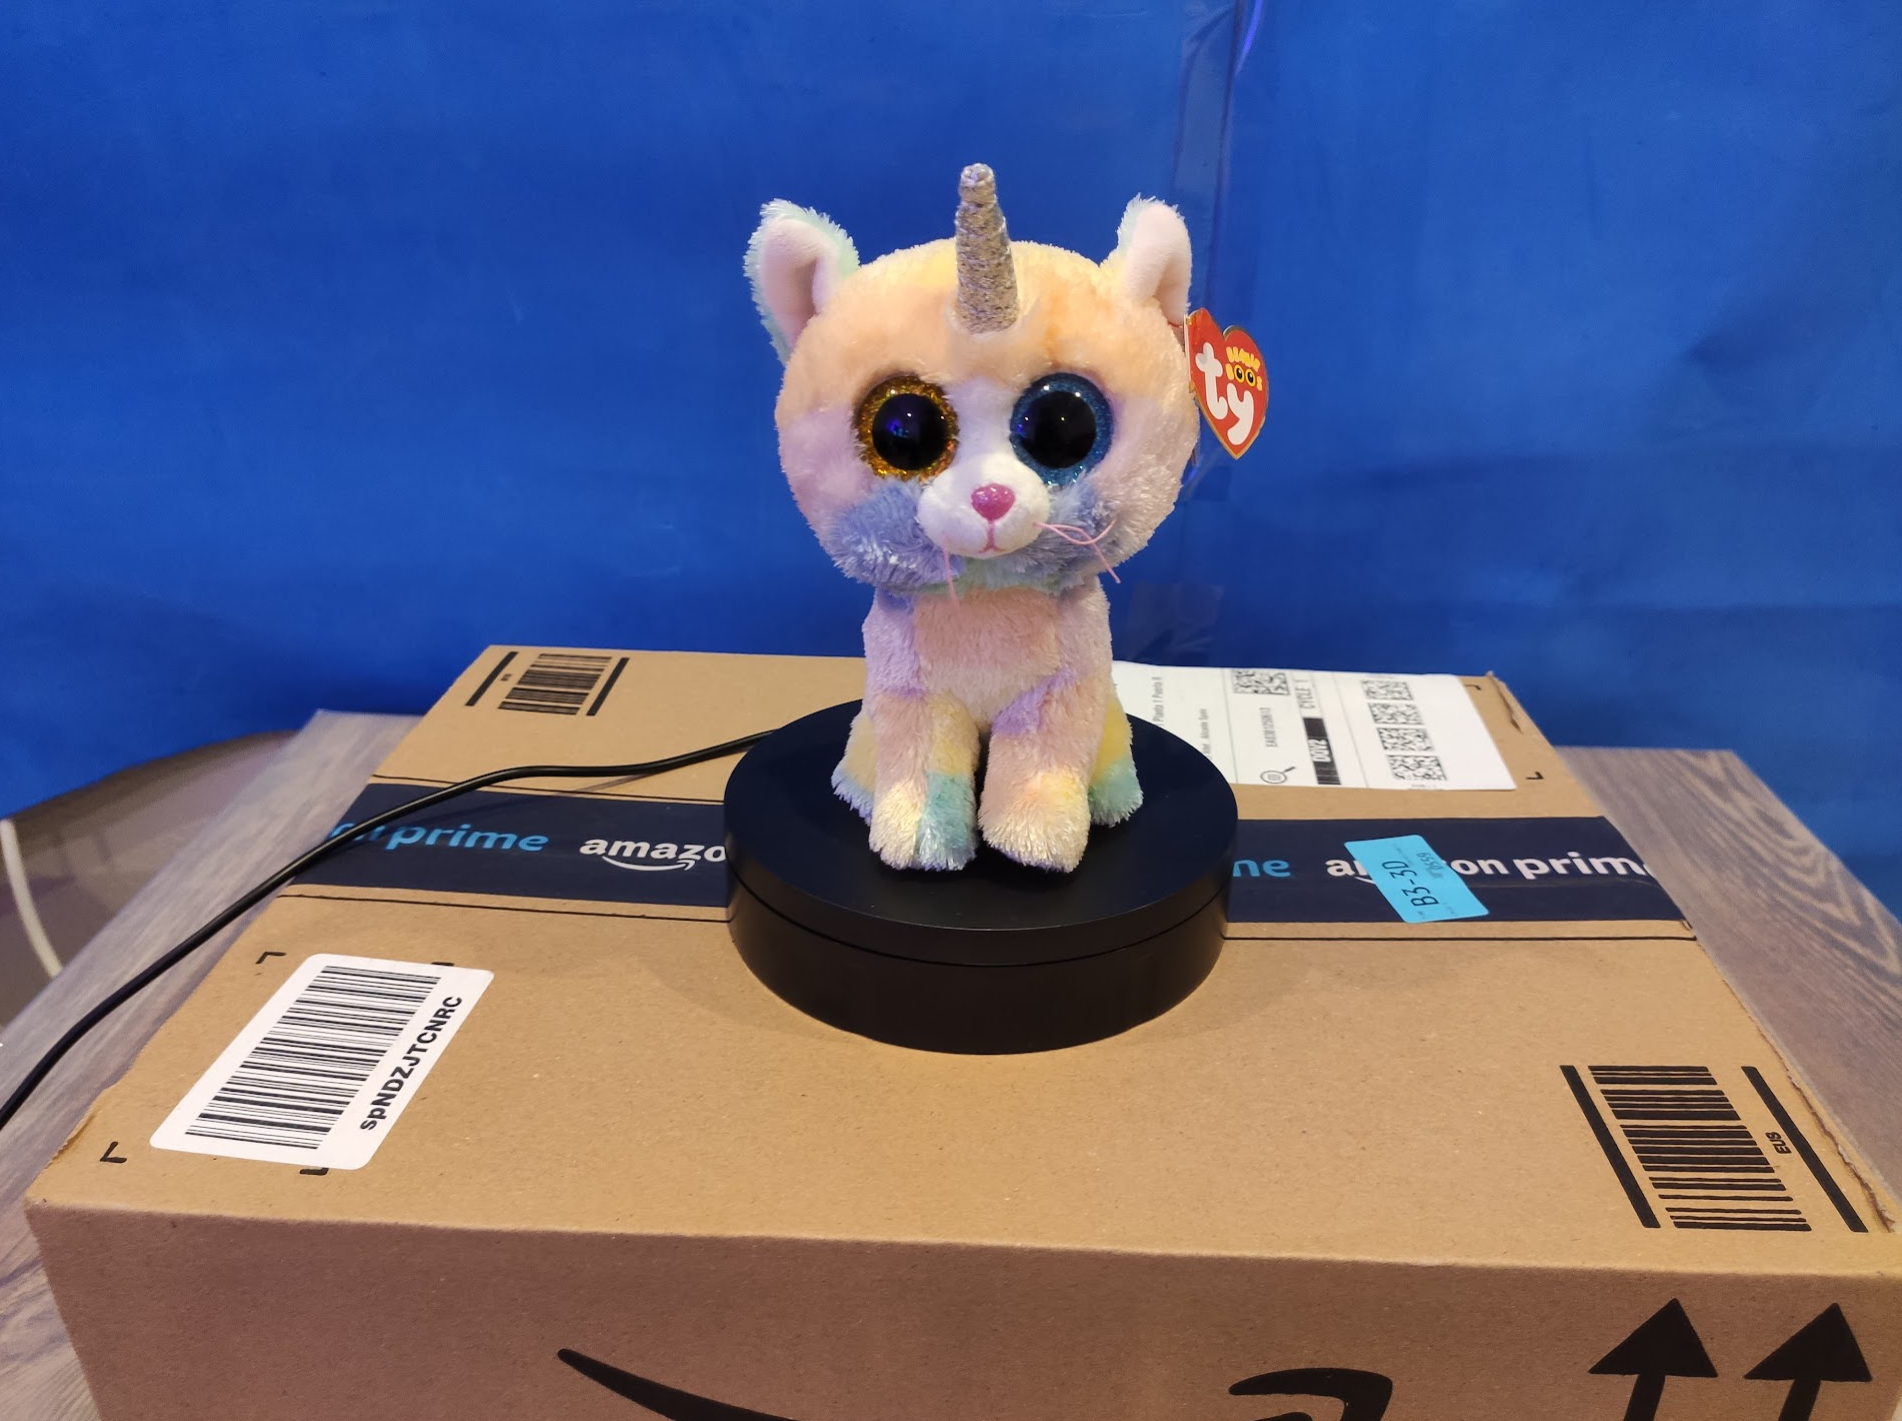
\includegraphics[height=3.5cm]{archivos/experimentacion-gato.png}
    \caption{Objeto de pruebas para reconstrucción 3D.}
    \label{fig:objetos-experimentacion}
\end{figure}

\section{Herramientas para visualizar las nubes de puntos}

Intel RealSense Viewer es una herramienta oficial de Intel para los sensores RealSense.
Con esta aplicación se puede visualizar la adquisición de la cámara en tiempo real, como se puede ver en la Figura \ref{fig:realsense-viewer-ejemplo}.
Tiene muchas herramientas y configuraciones que pueden ser útiles para experimentar con la cámara.

\begin{figure}[h]
    \centering
    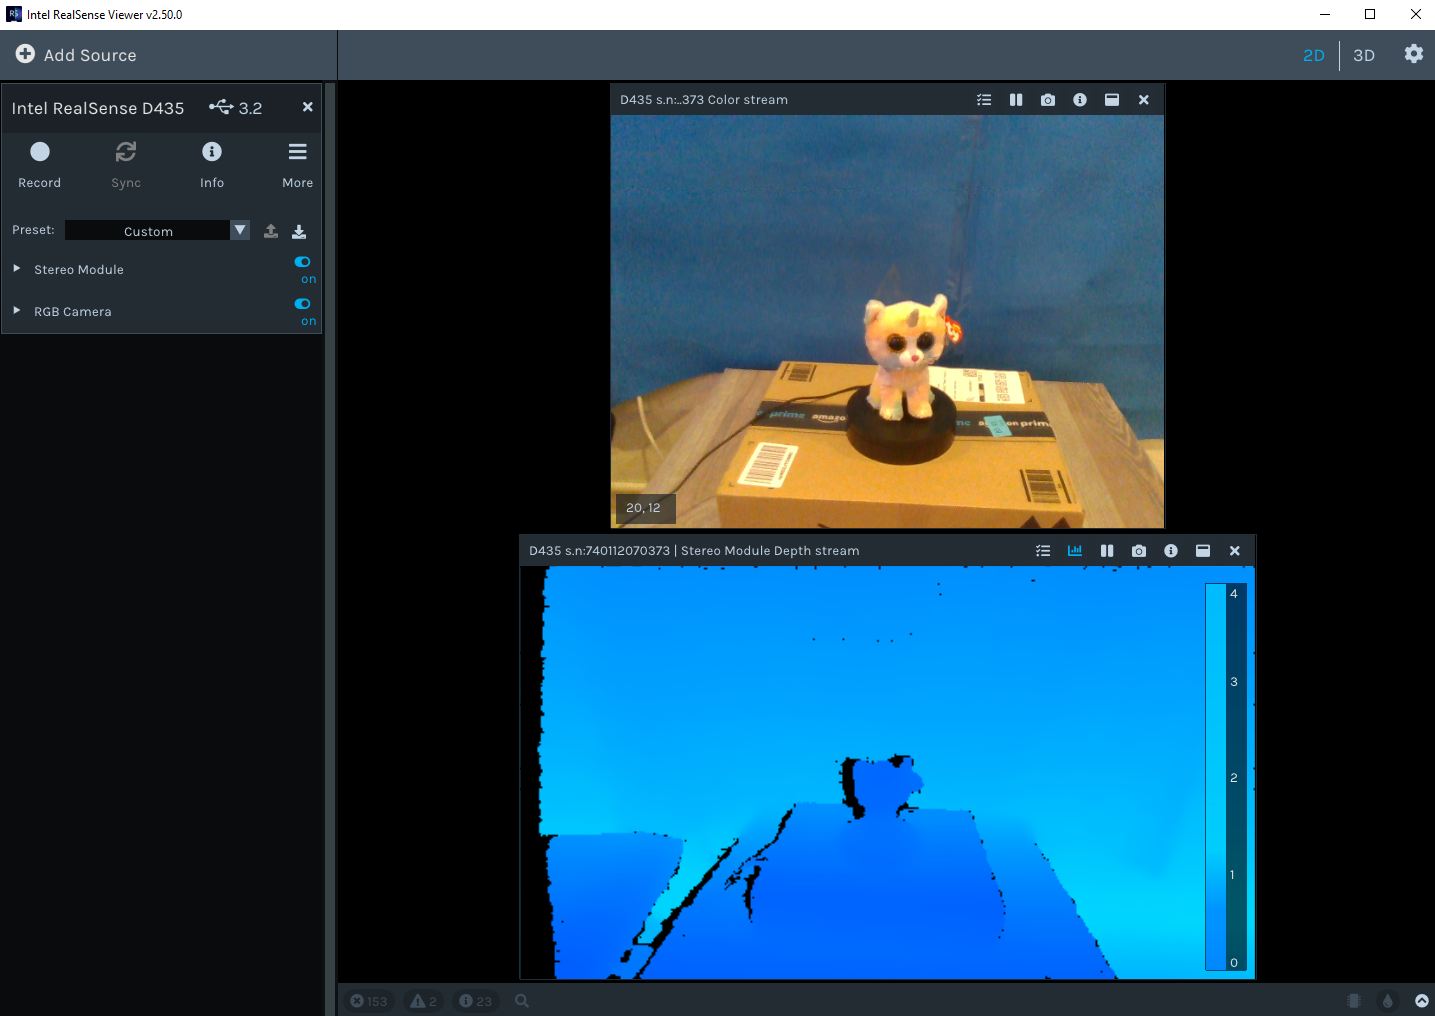
\includegraphics[height=7cm]{archivos/intel-realsense-viewer.png}
    \caption{Captura de pantalla de Intel RealSense Viewer.}
    \label{fig:realsense-viewer-ejemplo}
\end{figure}

Otra herramienta interesante es MeshLab. Meshlab un software de código abierto para el procesamiento y edición de mallas triangulares no estructuradas en 3D \citep{RCDCS13} \citep{LocalChapterEvents:ItalChap:ItalianChapConf2008:129-136}.
Este sistema tiene varias herramientas para la edición, optimización, inspección y renderización de mallas.
Ha sido muy útil debido a la comodidad y facilidad con la que representa los datos en pantalla.
En la Figura \ref{fig:meshlab-ejemplo} podemos ver un ejemplo con tres nubes de puntos.
Fácilmente podemos diferenciar cada nube de puntos otorgándoles un color distinto y solapándolos.
Además, MeshLab contiene herramientas interesantes para el análisis de los resultados, pudiendo convertir las nubes de puntos resultantes en mallas \gls{3d} con mejor visualización \citep{kazhdan2013screened}.

\begin{figure}[h]
    \centering
    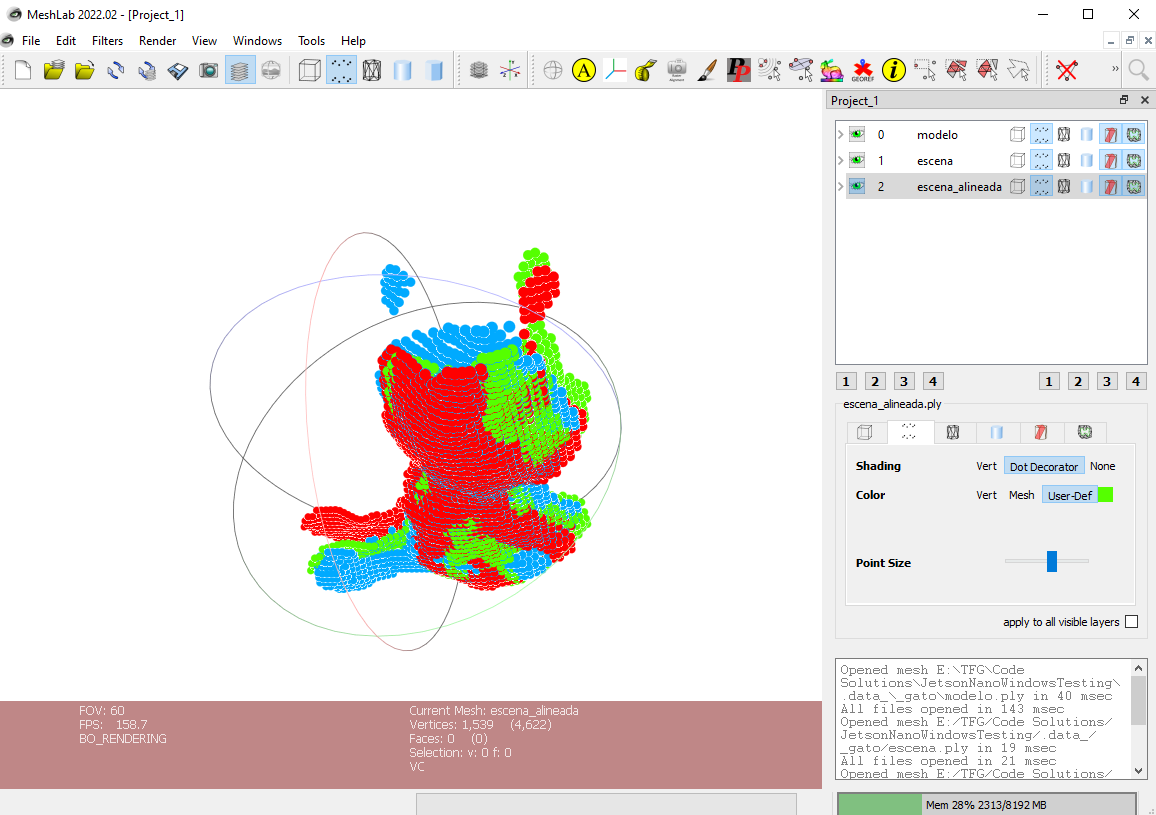
\includegraphics[height=7cm]{archivos/meshlab.png}
    \caption{Captura de pantalla de MeshLab con 3 nubes de puntos.}
    \label{fig:meshlab-ejemplo}
\end{figure}

\section{Resultados entre un modelo y una escena}

Para probar la solución del algoritmo \gls{icp} entre un modelo y una escena, utilizaremos un objeto rígido que rote ligeramente entre una captura y otra.
Para ello, utilizaremos las capturas de la Figura \ref{fig:objetos-experimentacion-modelo-escena}.

\begin{figure}[h]
    \centering
    \begin{subfigure}[t]{0.33\textheight}
    	\centering
        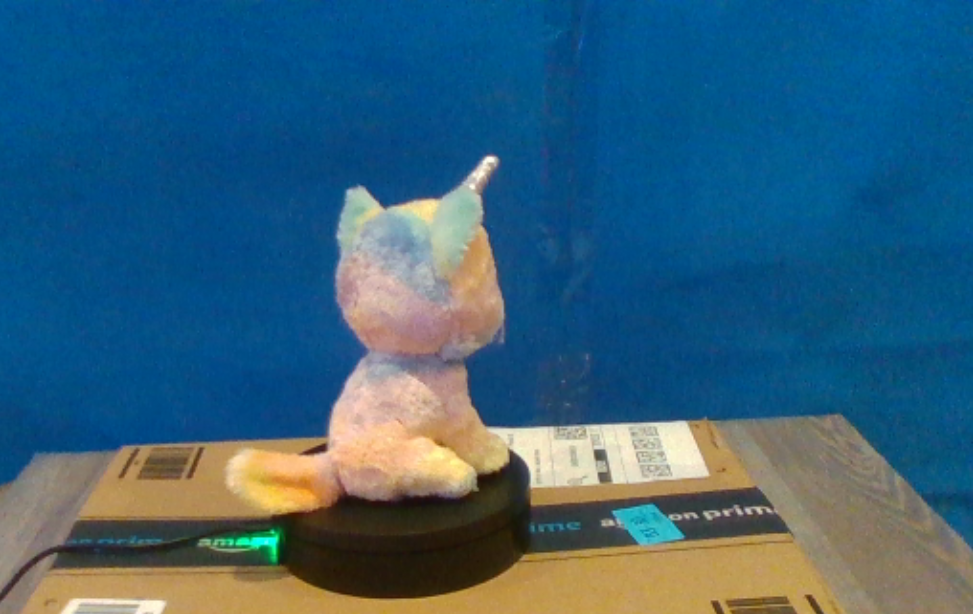
\includegraphics[height=3.5cm]{archivos/experimentacion-modelo.png}
        \caption{Modelo.}
    \end{subfigure}
    \begin{subfigure}[t]{0.33\textheight}
    	\centering
        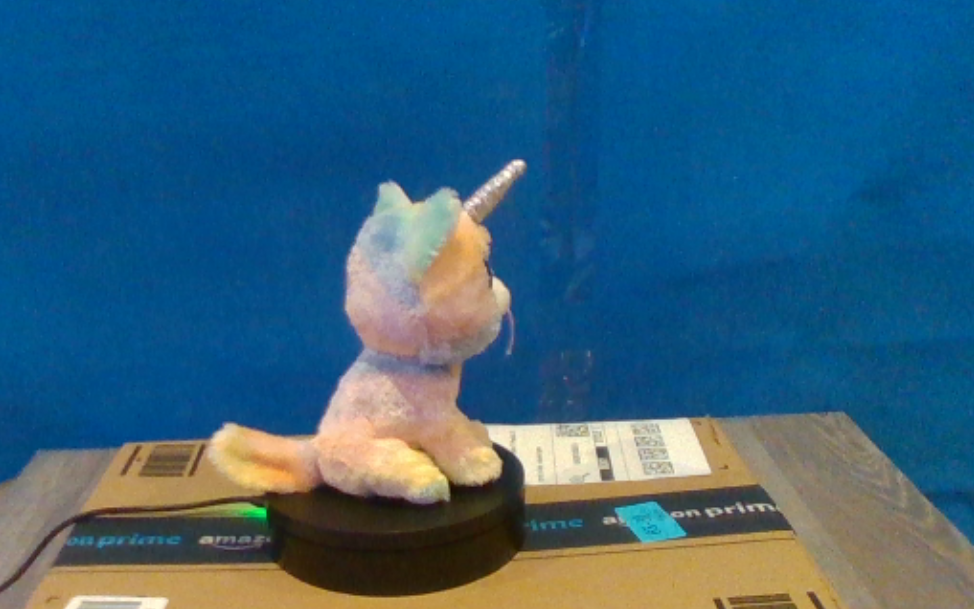
\includegraphics[height=3.5cm]{archivos/experimentacion-escena.png}
        \caption{Escena.}
    \end{subfigure}
    \caption{Ejemplo de alineación de una escena con un modelo.}
    \label{fig:objetos-experimentacion-modelo-escena}
\end{figure}

En la Figura \ref{fig:experimentacion-1} podemos ver los resultado de aplicar los algoritmo \gls{icp} de \gls{pcl}, CUDA-ICP y \gls{cpd}.
Para lograr estos resultados se ha establecido un máximo de 200 iteraciones en los algoritmos, y un límite de distancia máxima de correspondencias de 0.01m, ya que las correpondencias deben ser muy cercanas.
Como se puede observar en las subfiguras \ref{fig:experimentacion-1-alineado-icp} y \ref{fig:experimentacion-1-alineado-cuda} la convergencia ha funcionado bastante bien y ambos resultados son muy parecidos.
Se ha probado a utilizar el algoritmo \gls{cpd} con la funcionalidad no rígida, sin embargo los resultados no son tan satisfactorios como se puede ver en la subfigura \ref{fig:experimentacion-1-alineado-cpd}.
Además, cabe mencionar que los tiempos para lograr estos resultados han sido de 0.97s para \gls{icp}, 0.72s para CUDA-ICP y 87.3s para \gls{cpd}.
Por el coste computacional tan elevado y los resultado obtenidos tras diversas pruebas con \gls{cpd} se ha decidido abandonar la idea de una transformación no rígida para centrarnos en los buenos resultados que nos pueden llegar a dar \gls{icp} y CUDA-ICP.

\begin{figure}[h]
    \centering
    \begin{subfigure}[t]{0.33\textheight}
    	\centering
        
\includegraphics[height=5.5cm]{archivos/experimentacion-1-modelo.png}
        \caption{Nube de puntos modelo.}
    \end{subfigure}
    \begin{subfigure}[t]{0.33\textheight}
    	\centering
        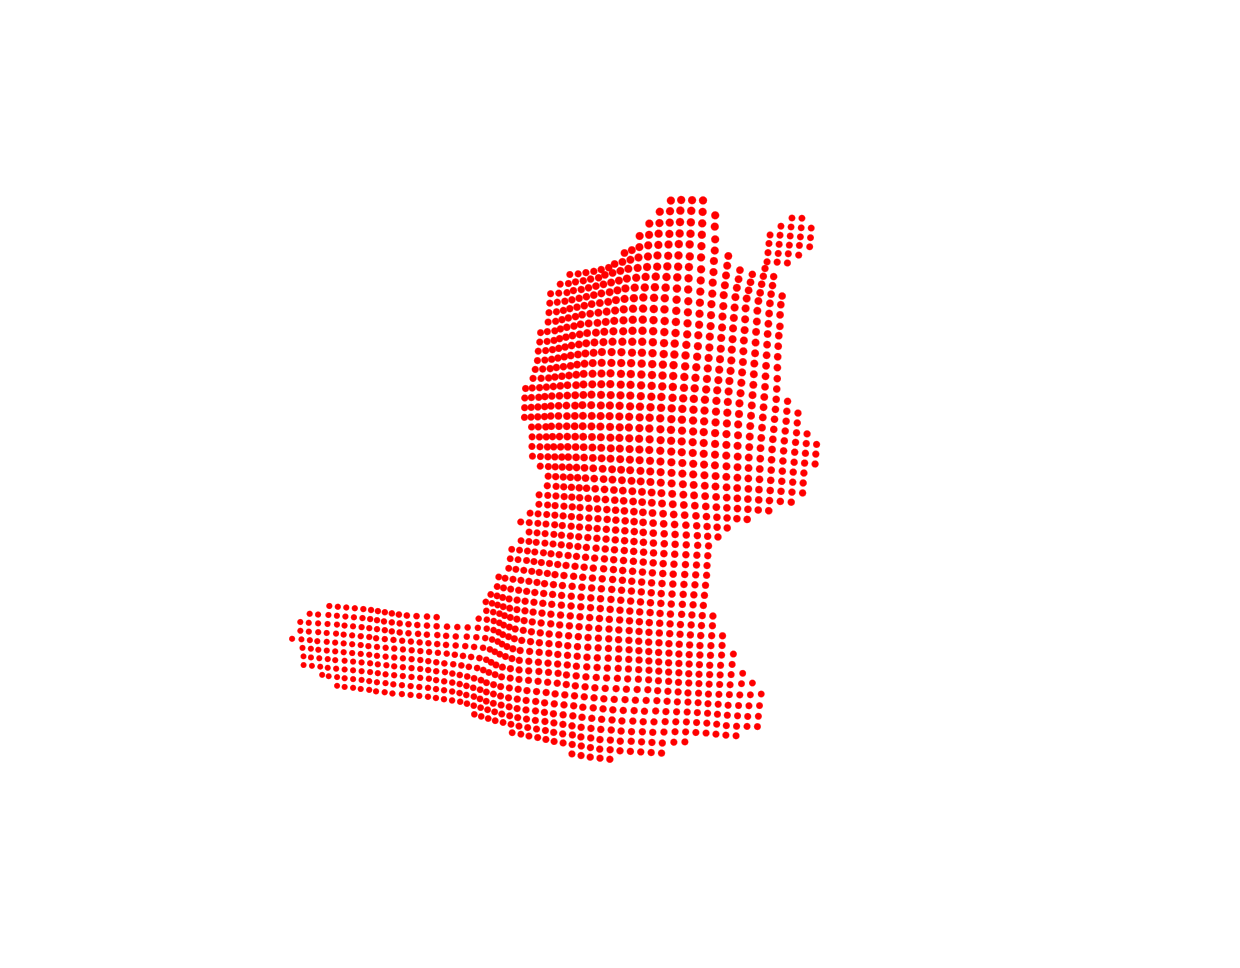
\includegraphics[height=5.5cm]{archivos/experimentacion-1-escena.png}
        \caption{Nube de puntos escena.}
    \end{subfigure}
    \begin{subfigure}[t]{0.33\textheight}
    	\centering
        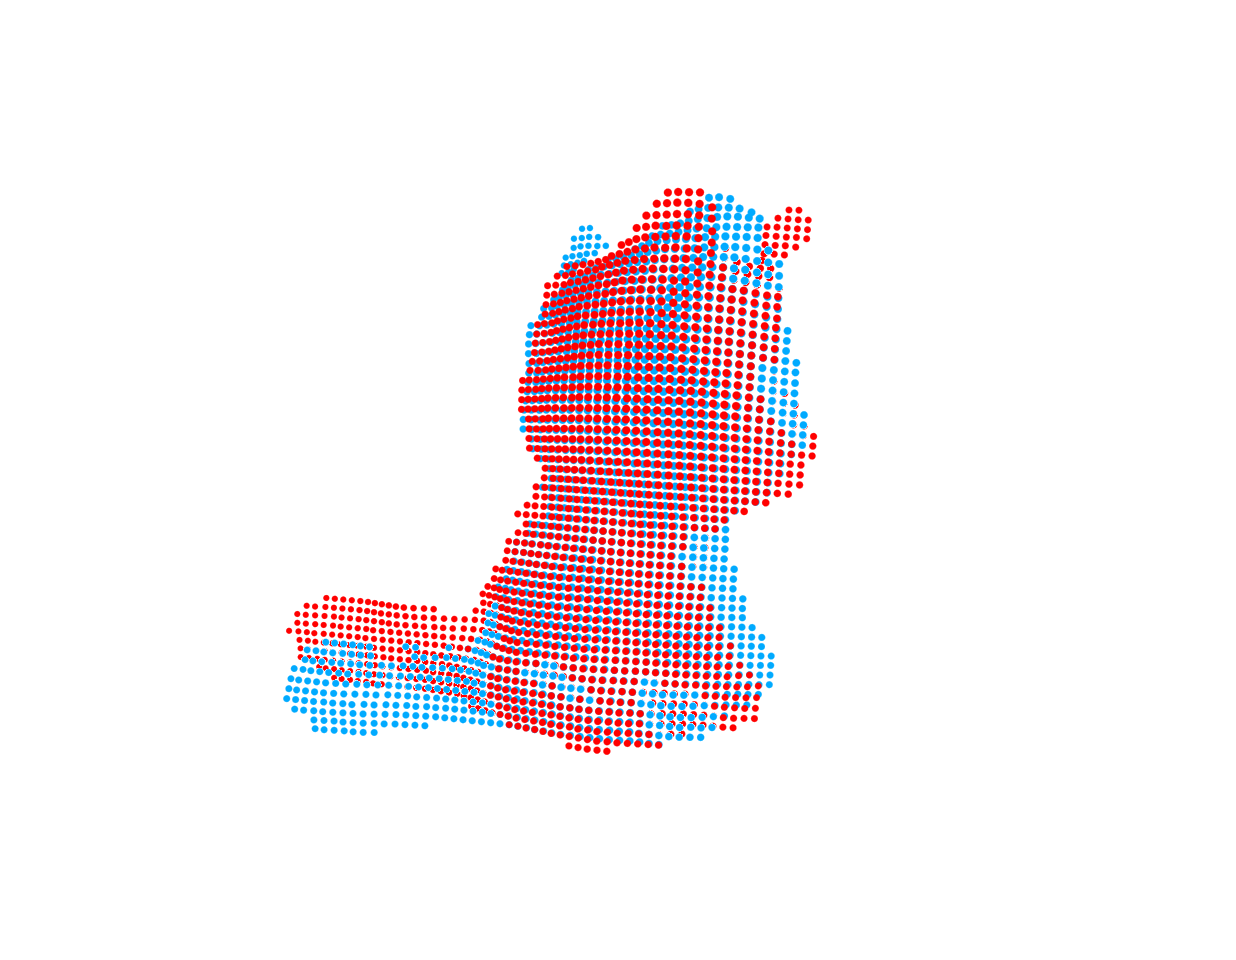
\includegraphics[height=5.5cm]{archivos/experimentacion-1-modelo-escena.png}
        \caption{Modelo y escena sin alinear.}
    \end{subfigure}
    \begin{subfigure}[t]{0.33\textheight}
    	\centering
        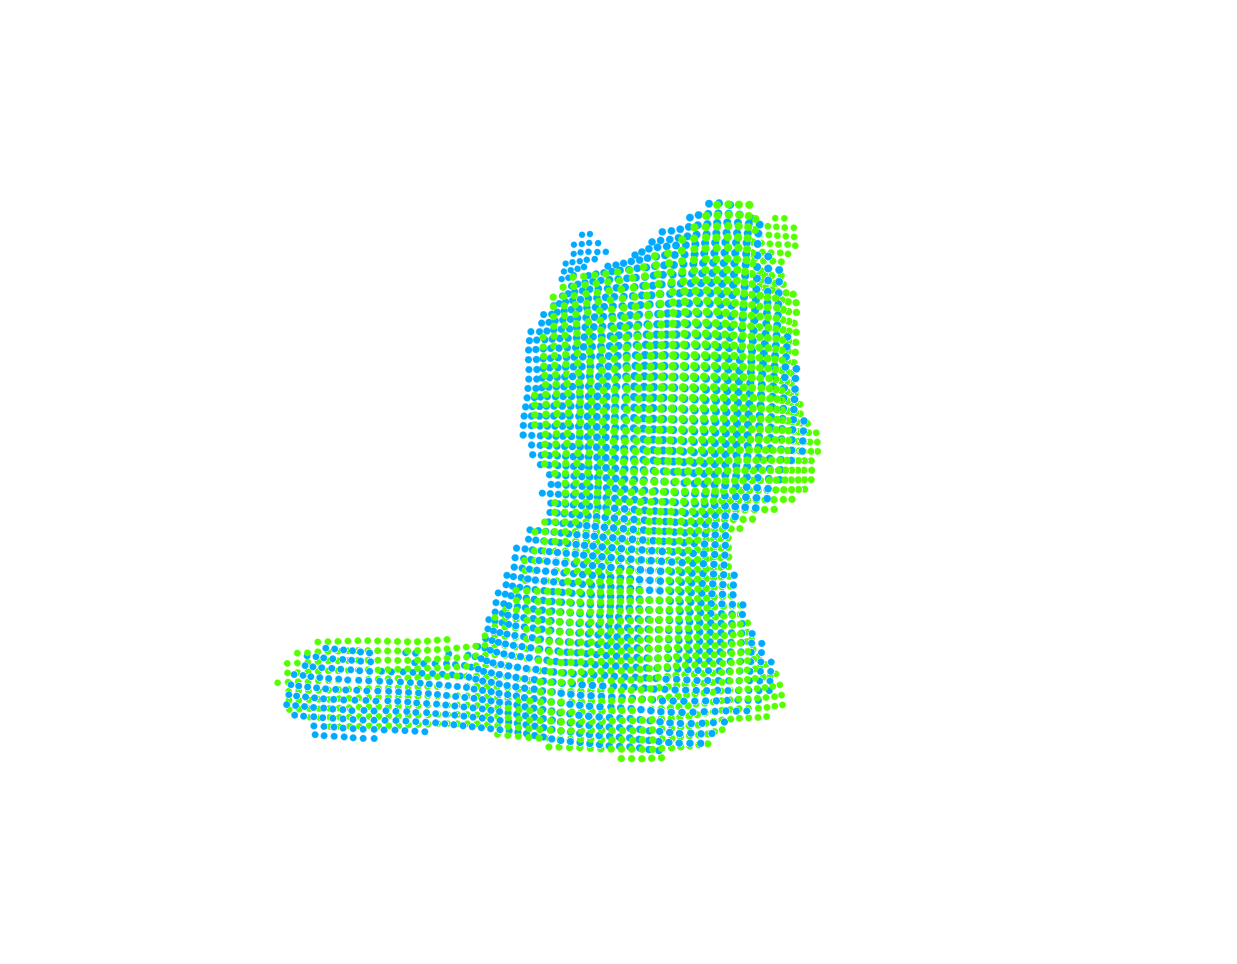
\includegraphics[height=5.5cm]{archivos/experimentacion-1-alineado-icp.png}
        \caption{Alineamiento con ICP.}
        \label{fig:experimentacion-1-alineado-icp}
    \end{subfigure}
    \begin{subfigure}[t]{0.33\textheight}
    	\centering
        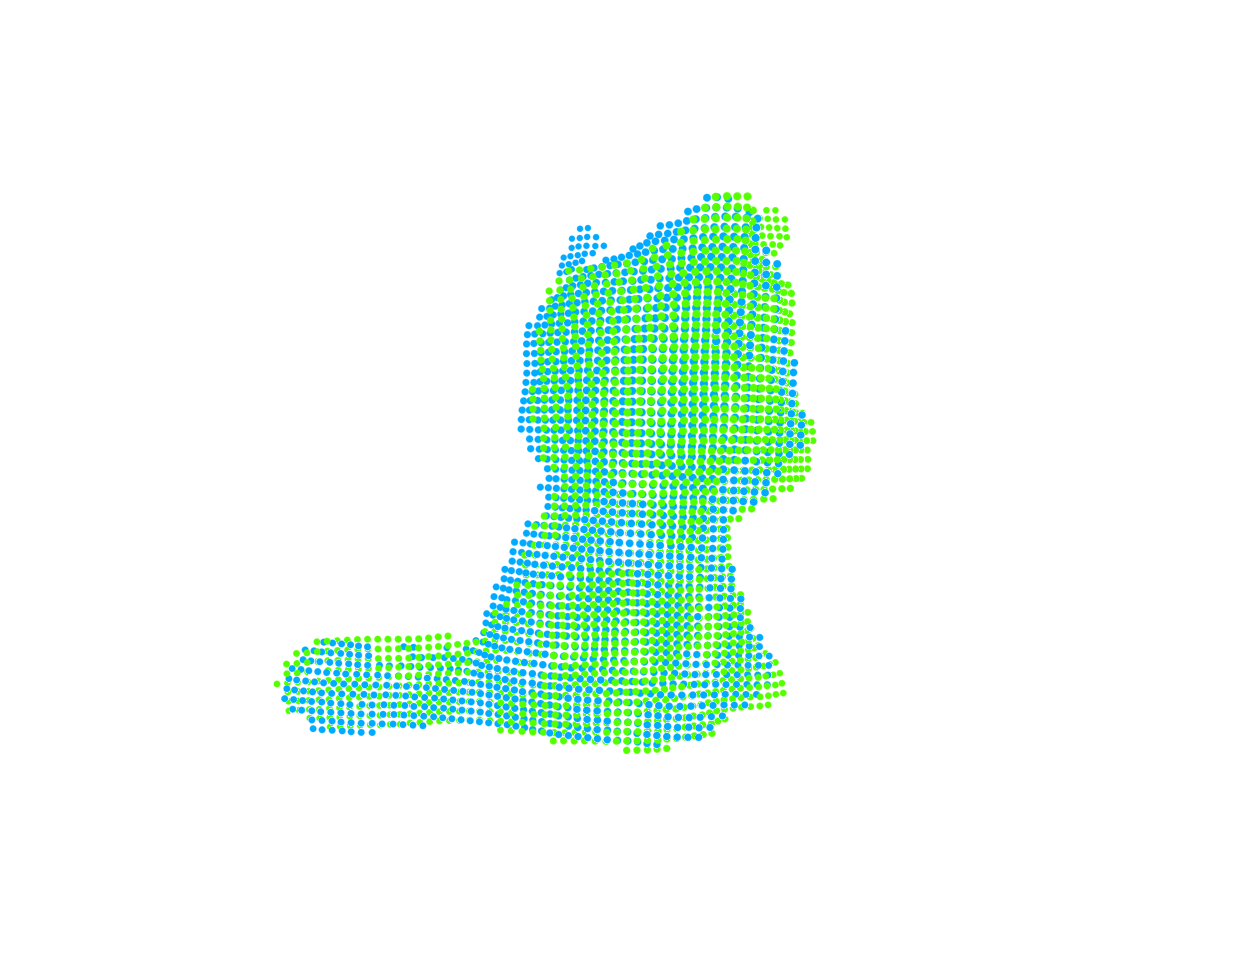
\includegraphics[height=5.5cm]{archivos/experimentacion-1-alineado-cuda.png}
        \caption{Alineamiento con CUDA-ICP.}
        \label{fig:experimentacion-1-alineado-cuda}
    \end{subfigure}
    \begin{subfigure}[t]{0.33\textheight}
    	\centering
        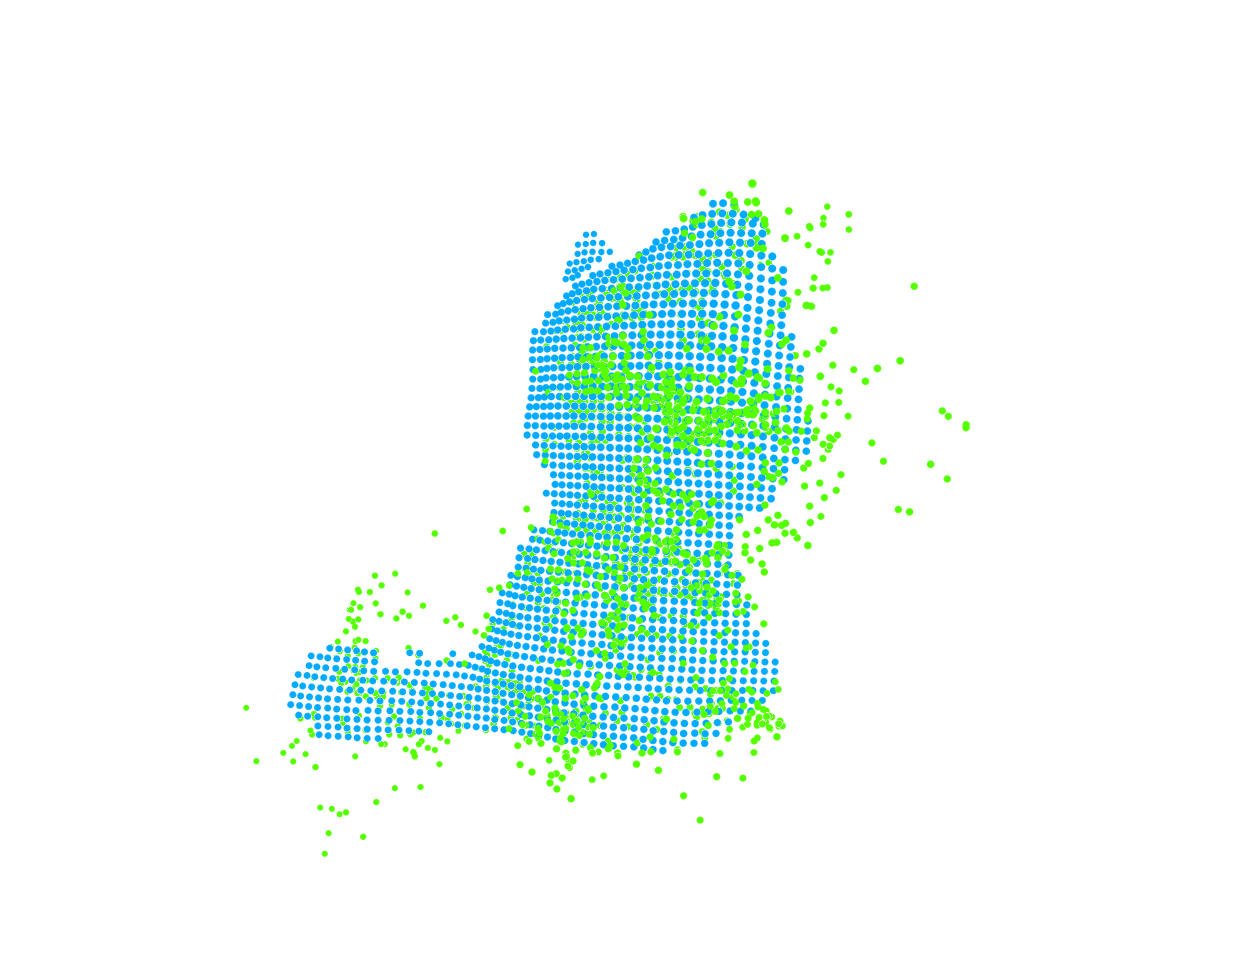
\includegraphics[height=5.5cm]{archivos/experimentacion-1-alineado-cpd.png}
        \caption{Alineamiento con CPD.}
        \label{fig:experimentacion-1-alineado-cpd}
    \end{subfigure}
    \caption{Resultados experimentación modelo y escena alineados.}
    \label{fig:experimentacion-1}
\end{figure}

\section{Resultados de la reconstrucción completa con un objeto}

Para la reconstrucción completa de un modelo \gls{3d} comenzaremos experimentando con el objeto de pruebas de la Figura \ref{fig:objetos-experimentacion} y, finalmente, se realizarán pruebas con el cuerpo humano.
En estas pruebas se utilizarán los algoritmos \gls{icp} y CUDA-ICP para comparar la calidad de la reconstrucción y los tiempos empleados en el dispositivo Jetson Nano.
Comenzaremos con el objeto de pruebas que ya hemos utilizado anteriormente.

Tras la fase de adquisición y pre-procesamiento obtenemos las capturas desde distintos ángulos del objeto.
El objeto ha estado girando con velocidad constante en un plato giratorio que tarda 21 segundos en realizar una vuelta 360º y para la fase de adquisición se ha establecido que el sensor capture imágenes cada 0.5 segundos.
Por tanto, obtenemos un total de 42 capturas del objeto.
A continuación, la primera de estas capturas será interpretada como el modelo y el resto irán siendo alineadas consecutivamente, hasta tener la reconstrucción completa.

En las Figuras \ref{fig:resultados-reconstruccion-objeto-icp} y \ref{fig:resultados-reconstruccion-objeto-cuda} podemos ver los resultados de las reconstrucción con \gls{icp} y CUDA-ICP, respectivamente.
Las cuatro primeras imágenes muestran el resultado de la nube de puntos reconstruida completamente, las siguientes cuatro imágenes muestran la reconstrucción de una malla generada a partir de la nube de puntos.

En la Tabla \ref{tab:resultado-objeto} tenemos datos interesantes respecto a los tiempos de reconstrucción. En la primer columna se indica el número de iteración que está pasando, seguidamente se indica la cantidad de puntos que tenía la escena en esa iteración, a continuación se expresa el tiempo que ha tardado la iteración en alinearse utilizando \gls{icp} y el tiempo total acumulado, seguidamente los mismos tiempos para CUDA-ICP, y finalmente los porcentajes de mejora de velocidad usando CUDA-ICP frente a \gls{icp} respecto al tiempo que tarda la iteración en sí y respecto al tiempo total.

Tras analizar los resultados vemos que los tiempos de ejecución de CUDA-ICP son mucho más rápidos que el algoritmo \gls{icp}, por lo que hay una buena mejora al estar aprovechando los núcleos de la gráfica, sin embargo el resultado final no ha conseguido converger tan bien como lo ha hecho \gls{icp} en \gls{pcl}.

\begin{figure}[h]
    \centering
    \begin{subfigure}[t]{0.2\textheight}
    	\centering
        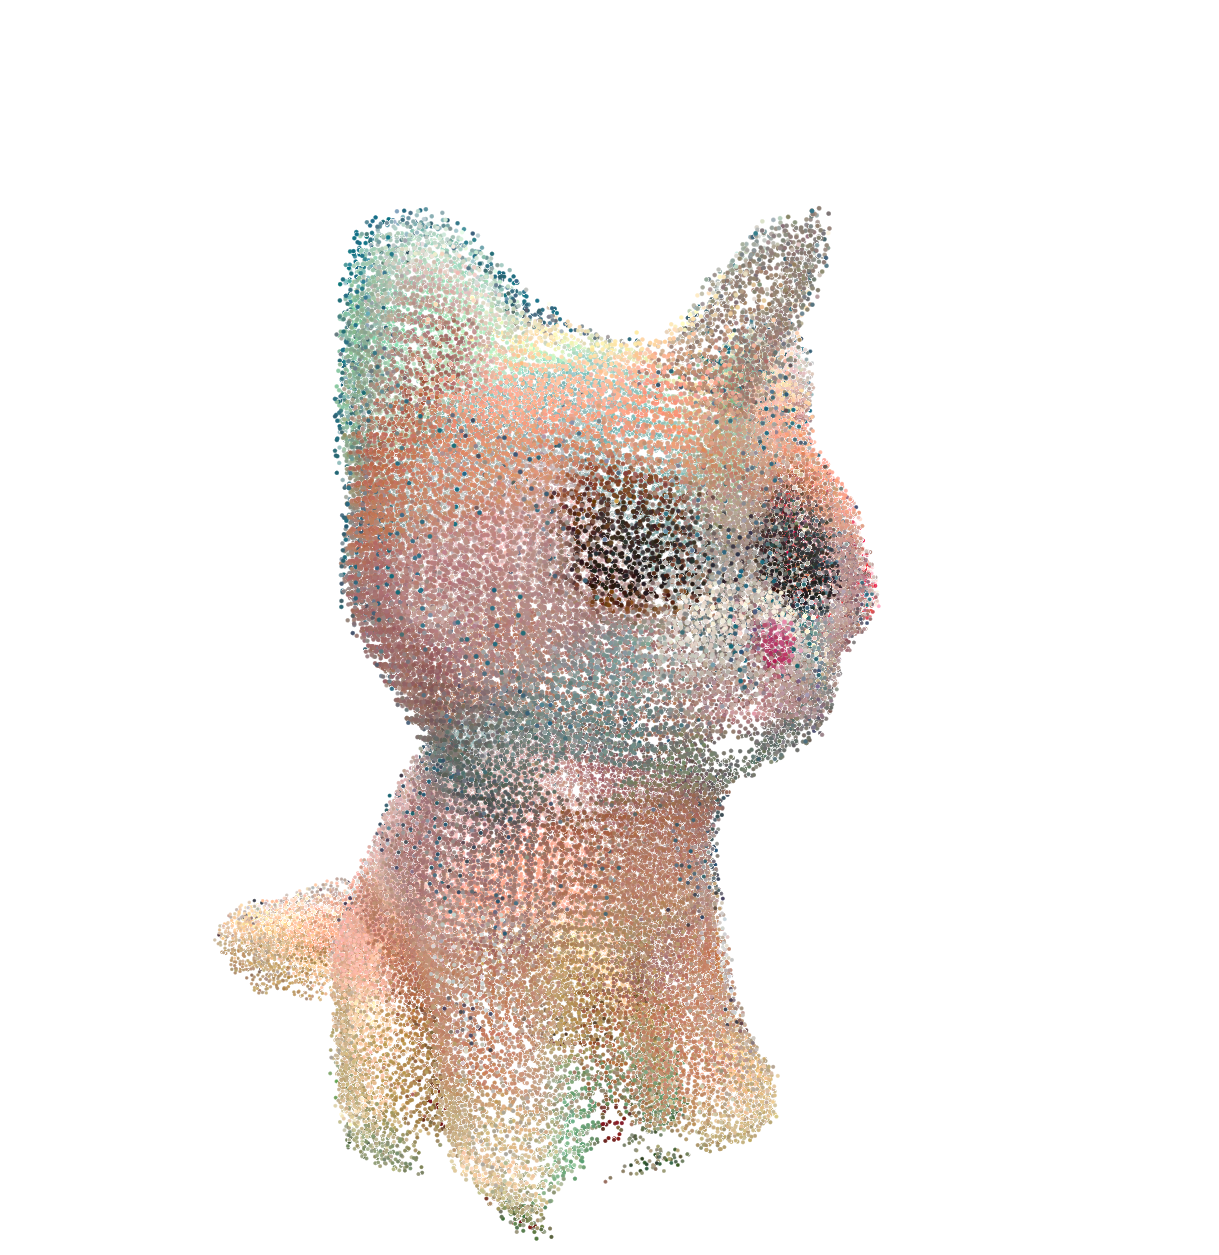
\includegraphics[height=4.5cm]{archivos/experimentacion-2-resultado-nube.png}
    \end{subfigure}
    \begin{subfigure}[t]{0.2\textheight}
    	\centering
        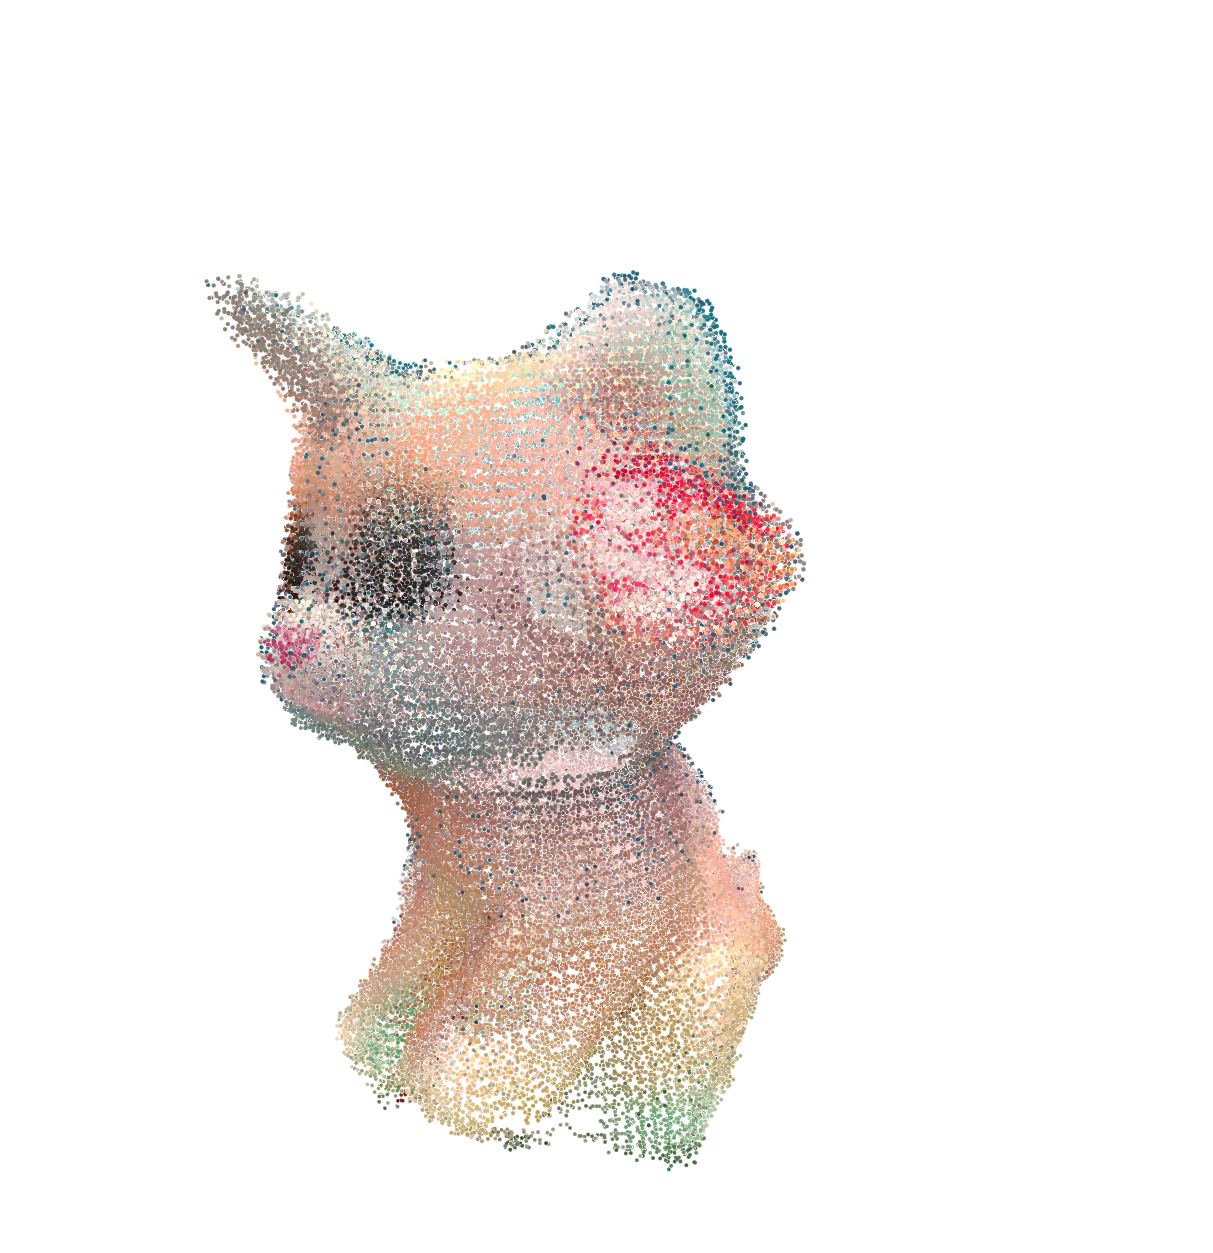
\includegraphics[height=4.5cm]{archivos/experimentacion-2-resultado-nube-2.png}
    \end{subfigure}
    \begin{subfigure}[t]{0.2\textheight}
    	\centering
        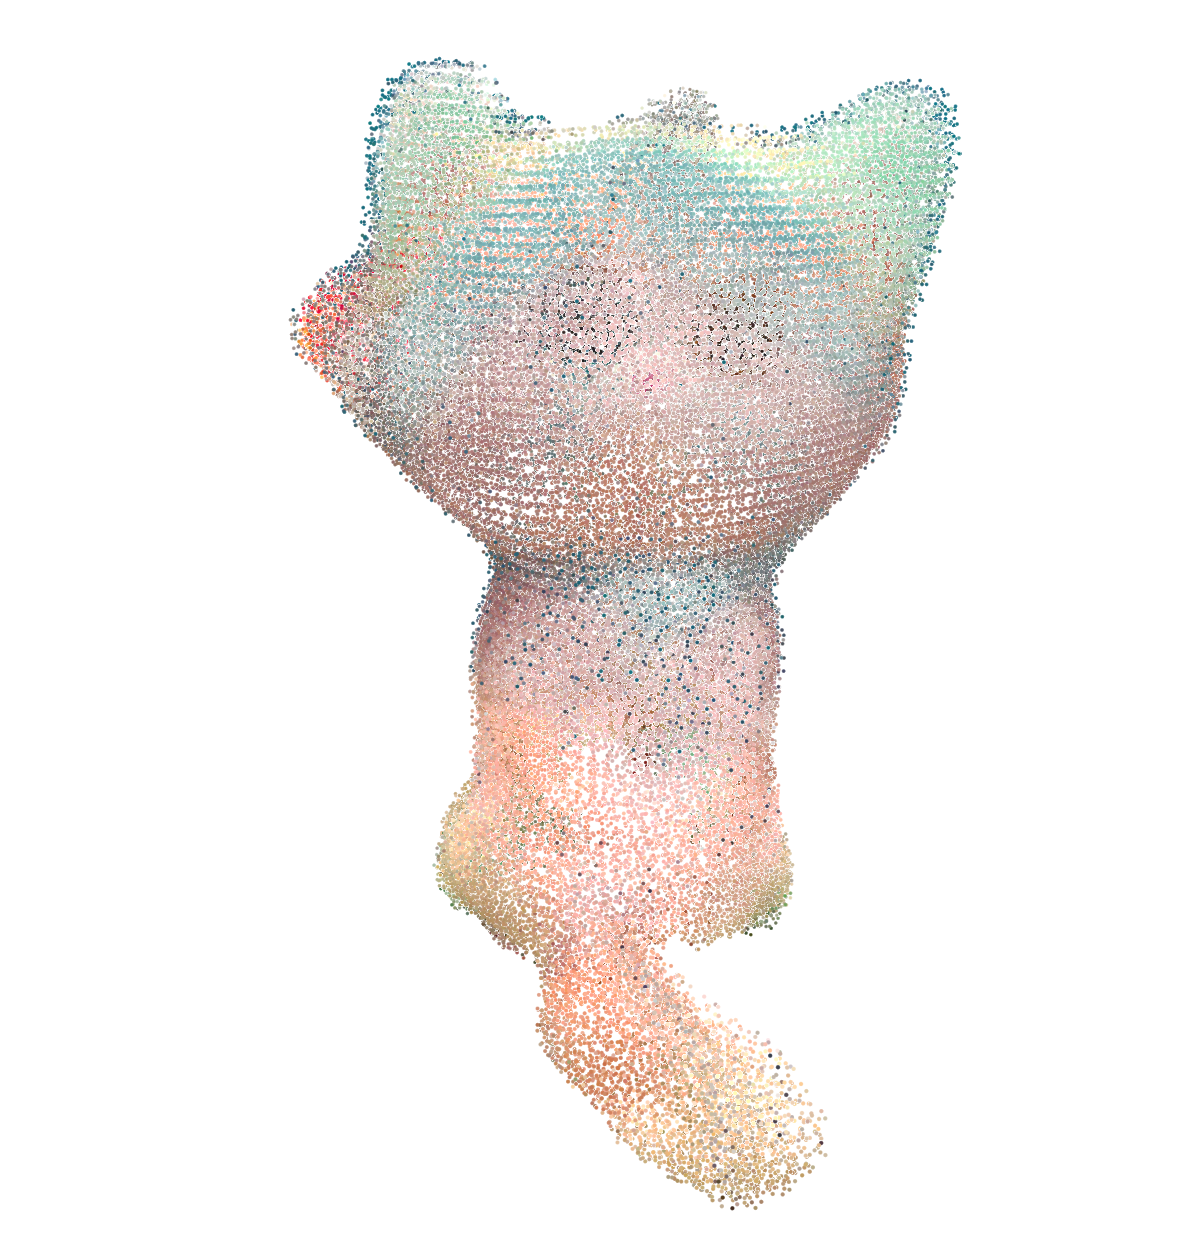
\includegraphics[height=4.5cm]{archivos/experimentacion-2-resultado-nube-3.png}
    \end{subfigure}
    \begin{subfigure}[t]{0.2\textheight}
    	\centering
        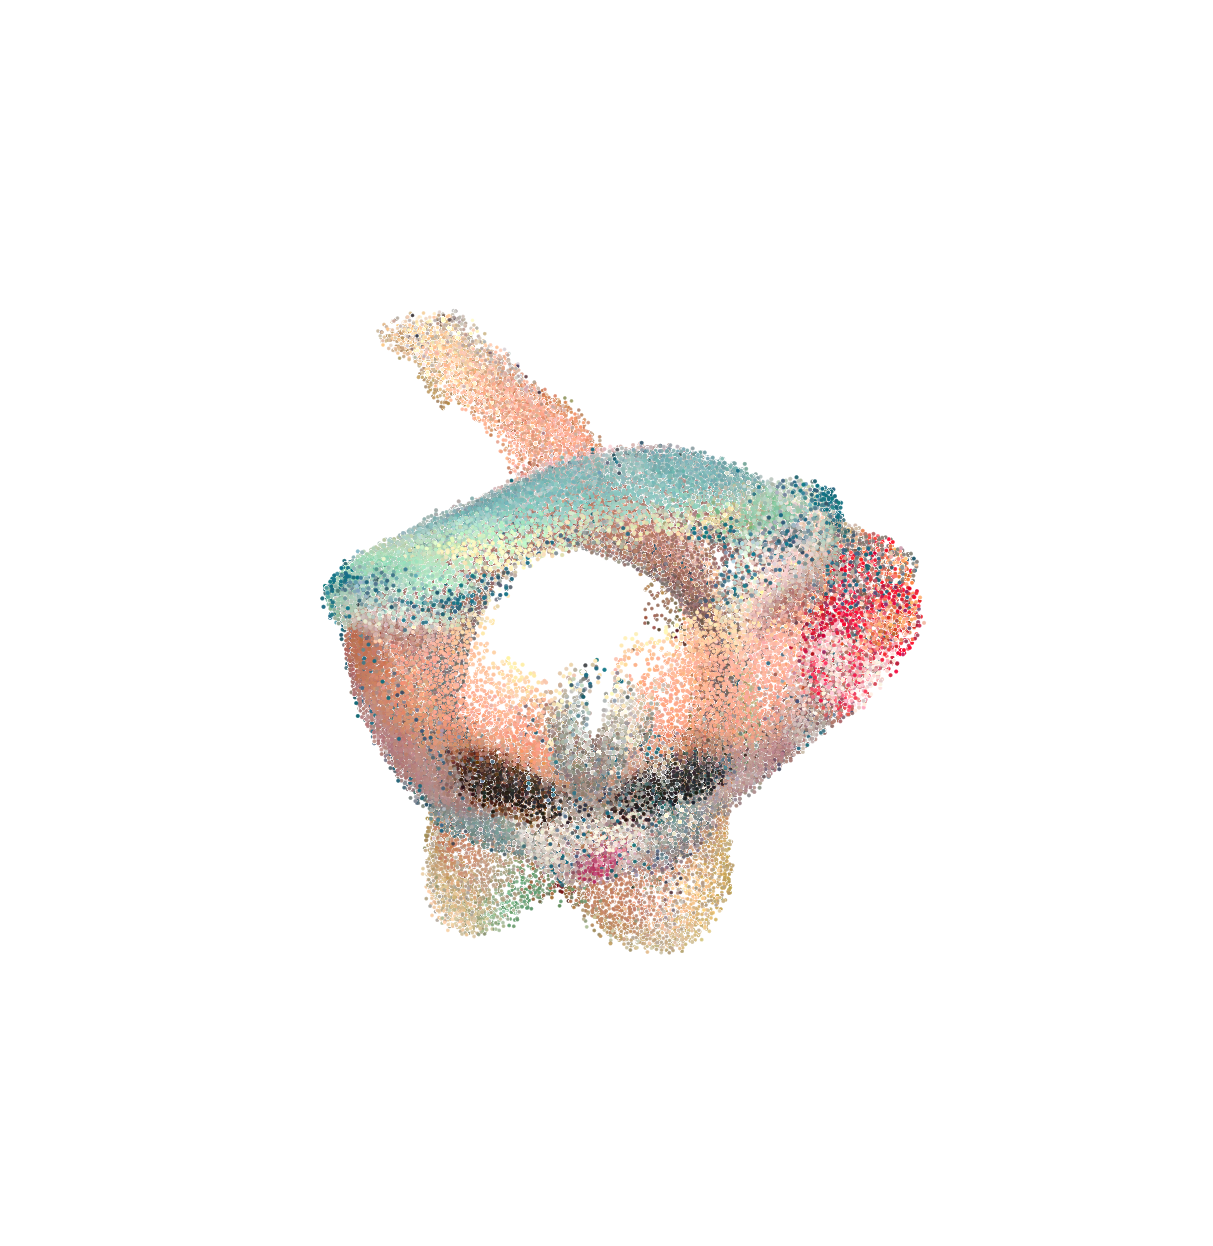
\includegraphics[height=4.5cm]{archivos/experimentacion-2-resultado-nube-4.png}
    \end{subfigure}
    \begin{subfigure}[t]{0.2\textheight}
    	\centering
        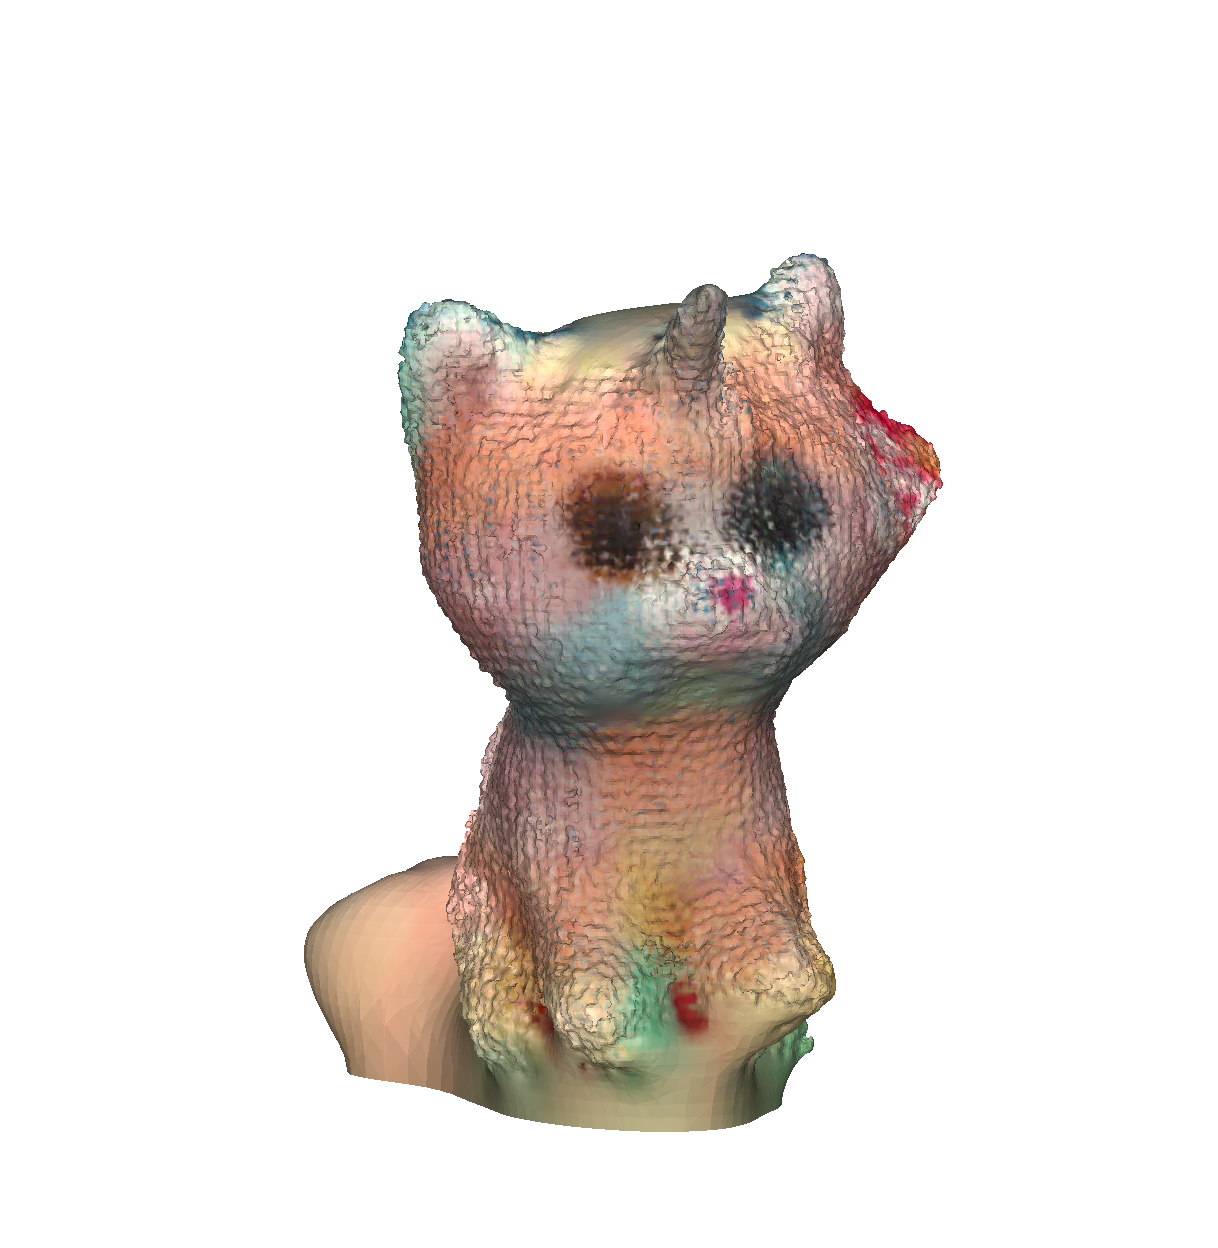
\includegraphics[height=4.5cm]{archivos/experimentacion-2-resultado-malla.png}
    \end{subfigure}
    \begin{subfigure}[t]{0.2\textheight}
    	\centering
        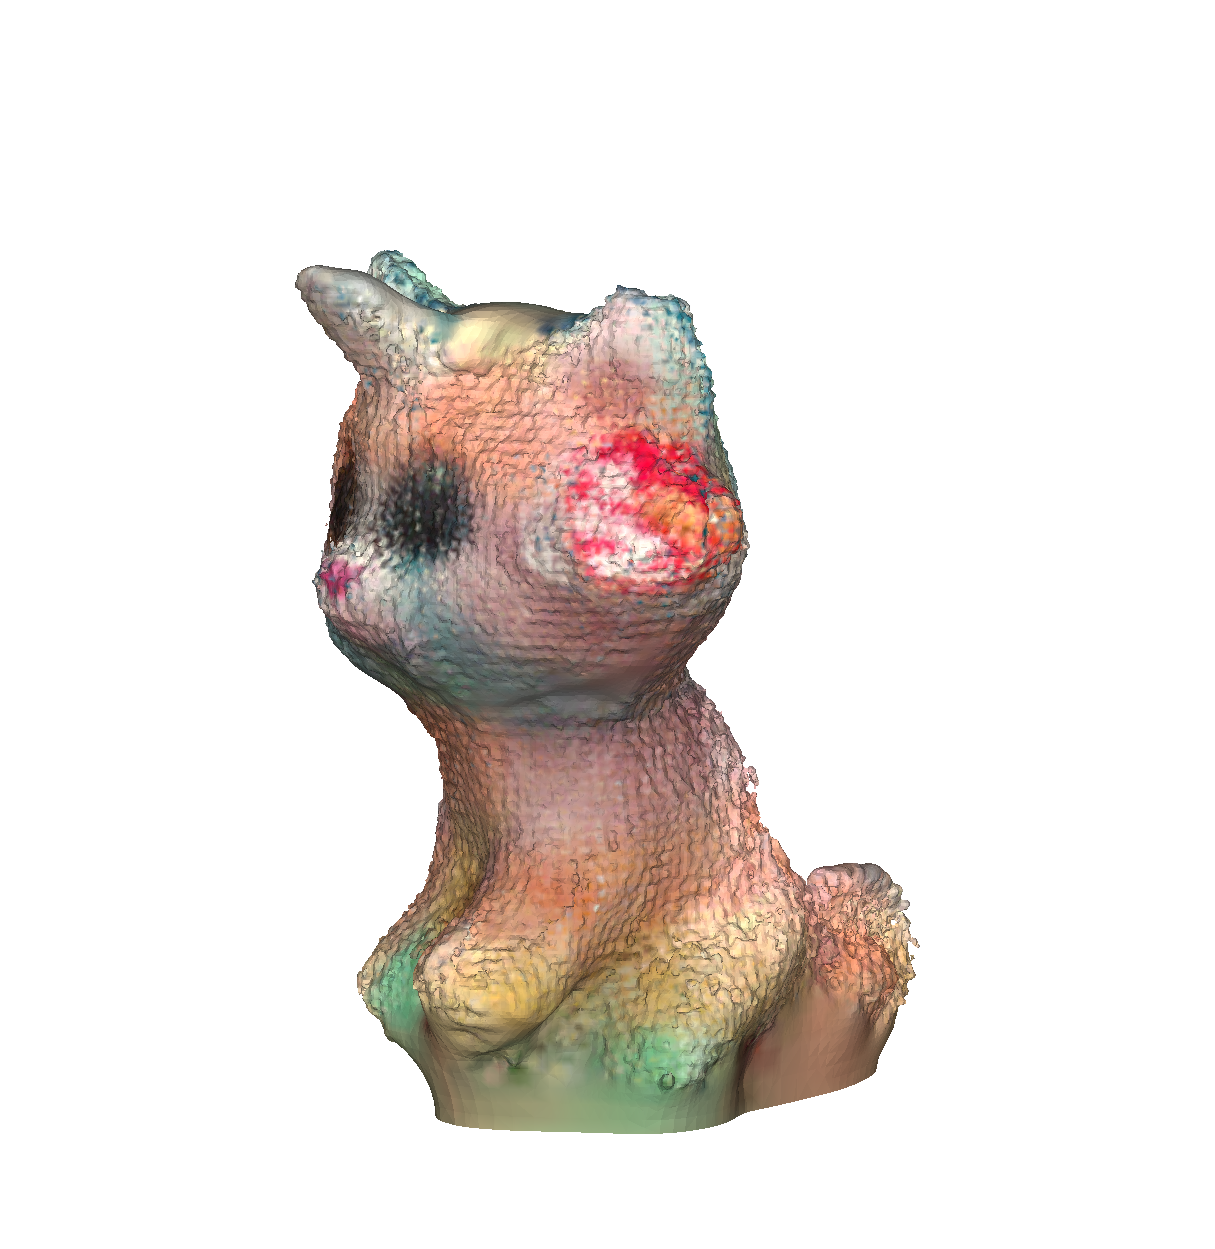
\includegraphics[height=4.5cm]{archivos/experimentacion-2-resultado-malla-2.png}
    \end{subfigure}
    \begin{subfigure}[t]{0.2\textheight}
    	\centering
        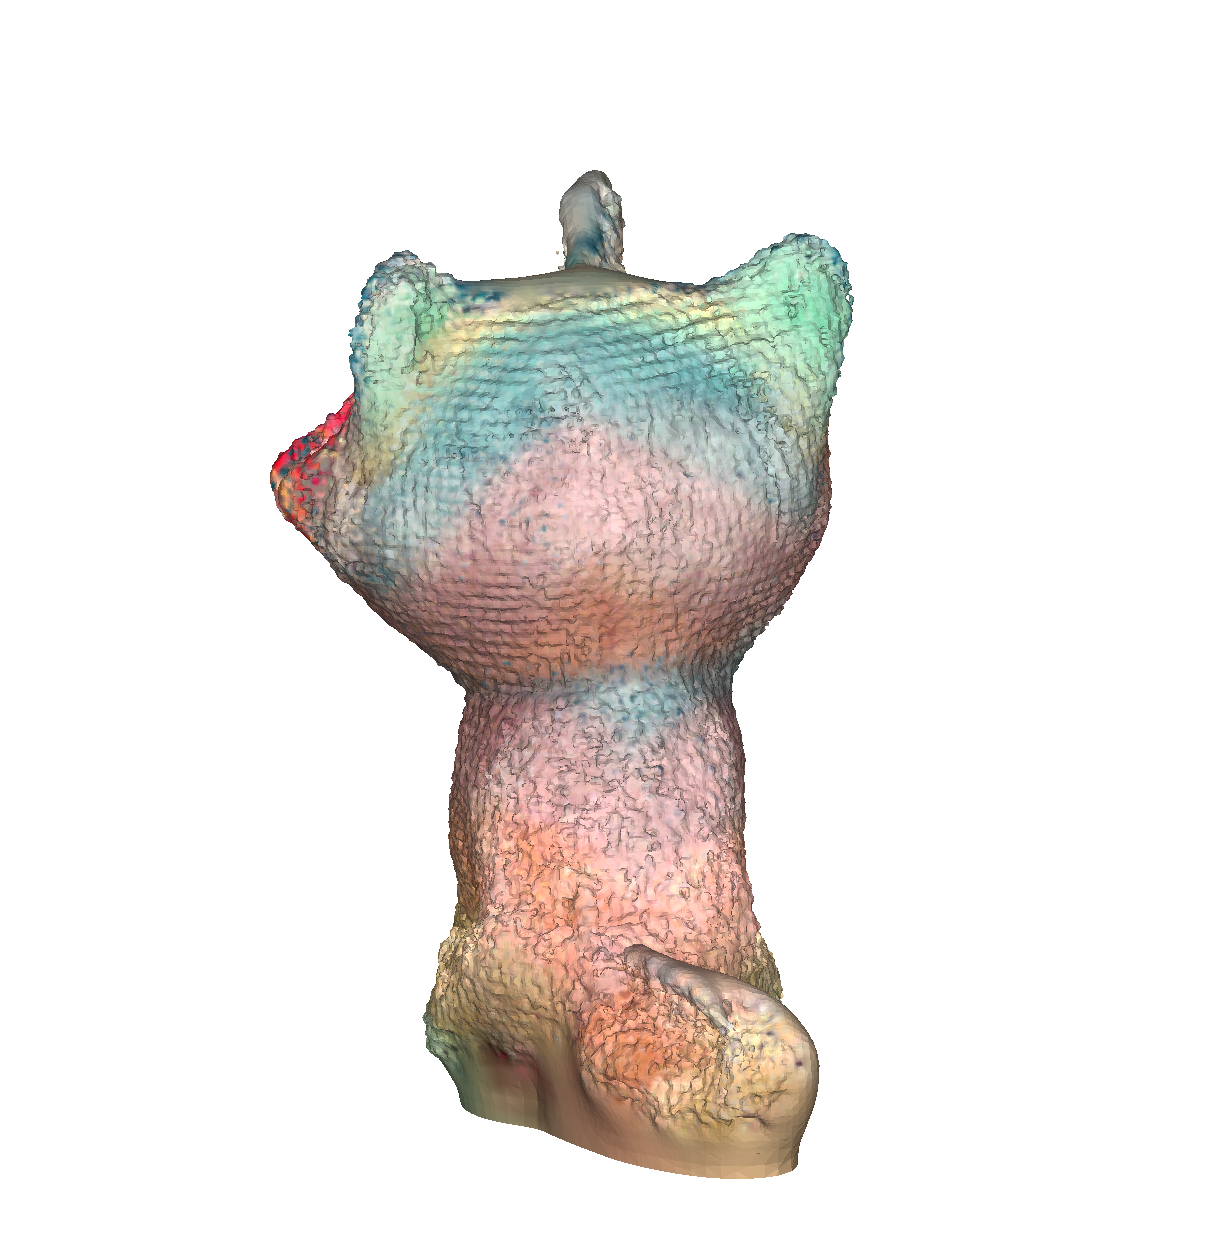
\includegraphics[height=4.5cm]{archivos/experimentacion-2-resultado-malla-3.png}
    \end{subfigure}
    \begin{subfigure}[t]{0.2\textheight}
    	\centering
        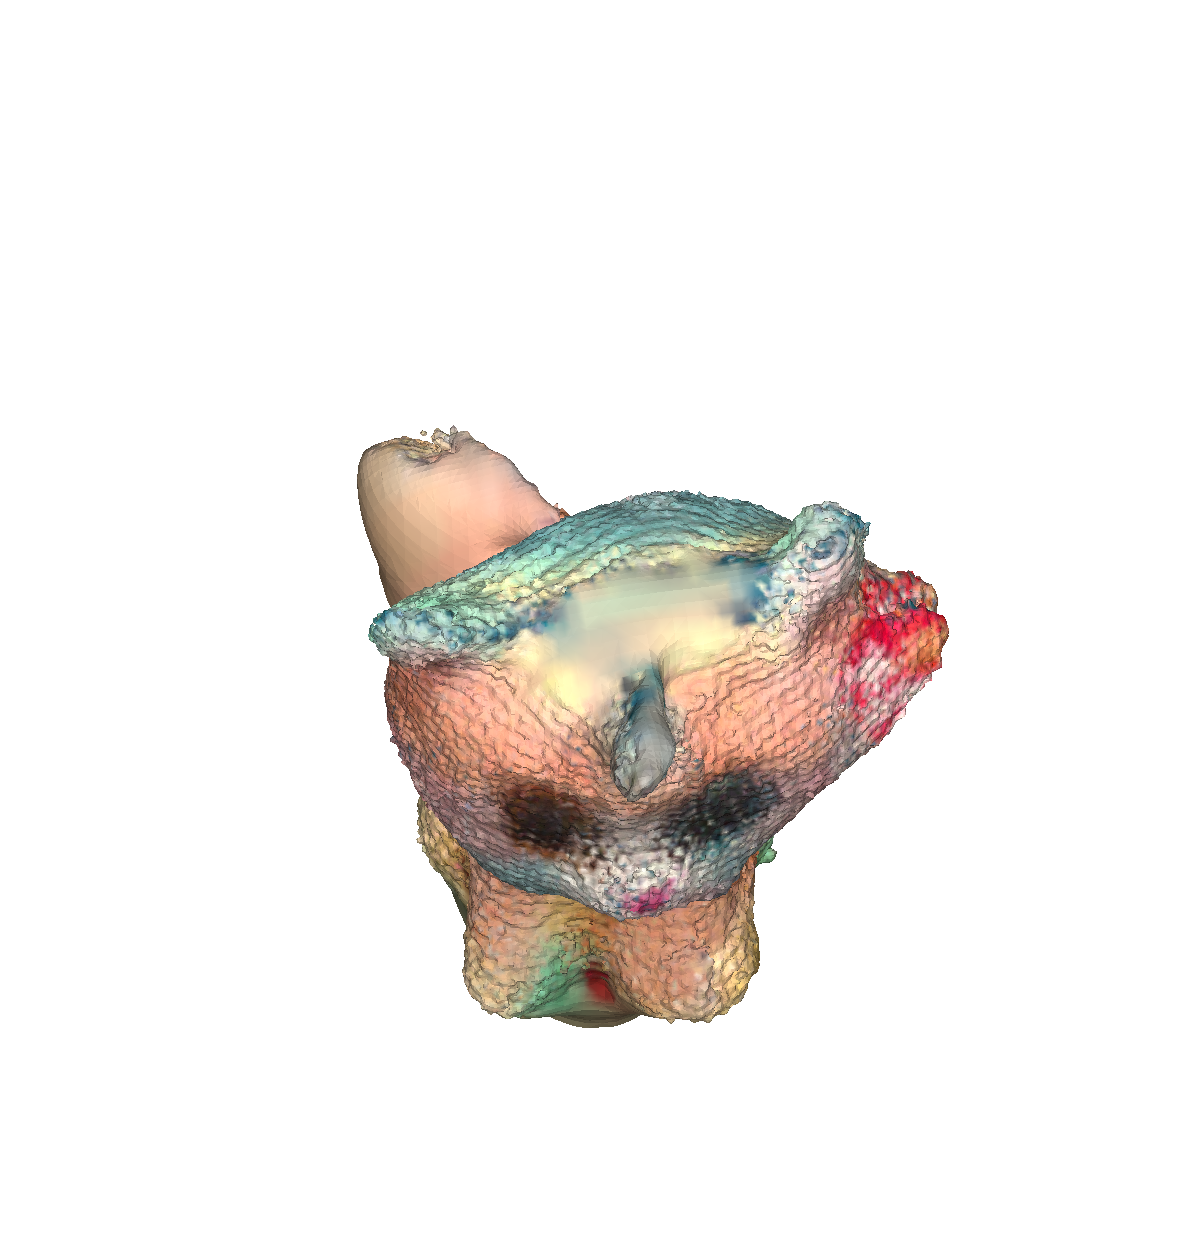
\includegraphics[height=4.5cm]{archivos/experimentacion-2-resultado-malla-4.png}
    \end{subfigure}
    \caption{Resultados de Reconstrucción 3D con objeto usando ICP.}
    \label{fig:resultados-reconstruccion-objeto-icp}
\end{figure}

\begin{figure}[h]
    \centering
    \begin{subfigure}[t]{0.2\textheight}
    	\centering
        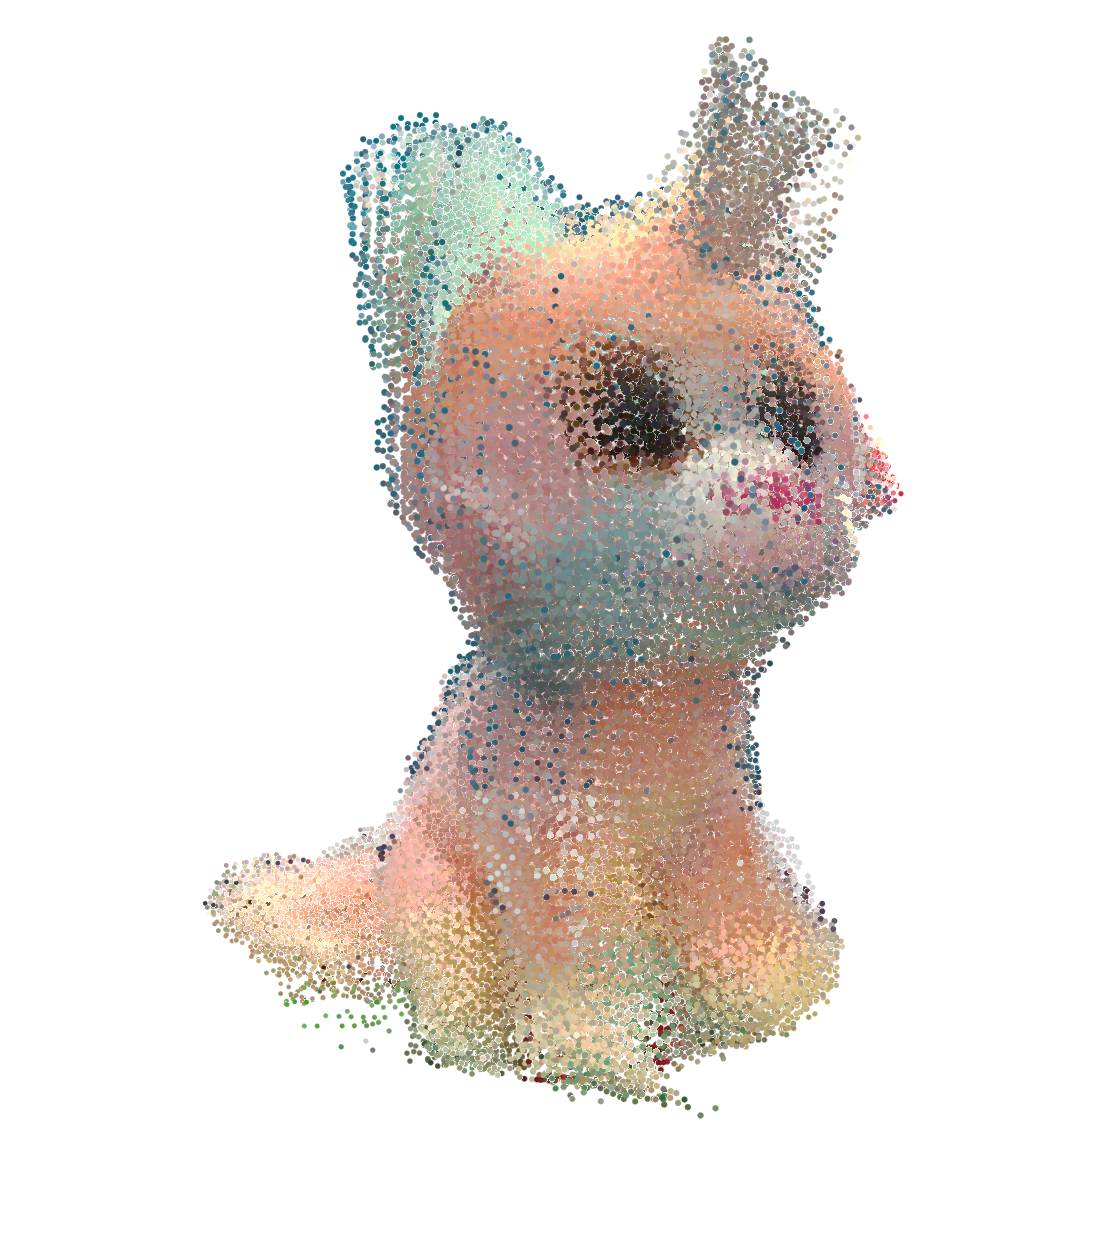
\includegraphics[height=4.5cm]{archivos/experimentacion-3-resultado-nube.png}
    \end{subfigure}
    \begin{subfigure}[t]{0.2\textheight}
    	\centering
        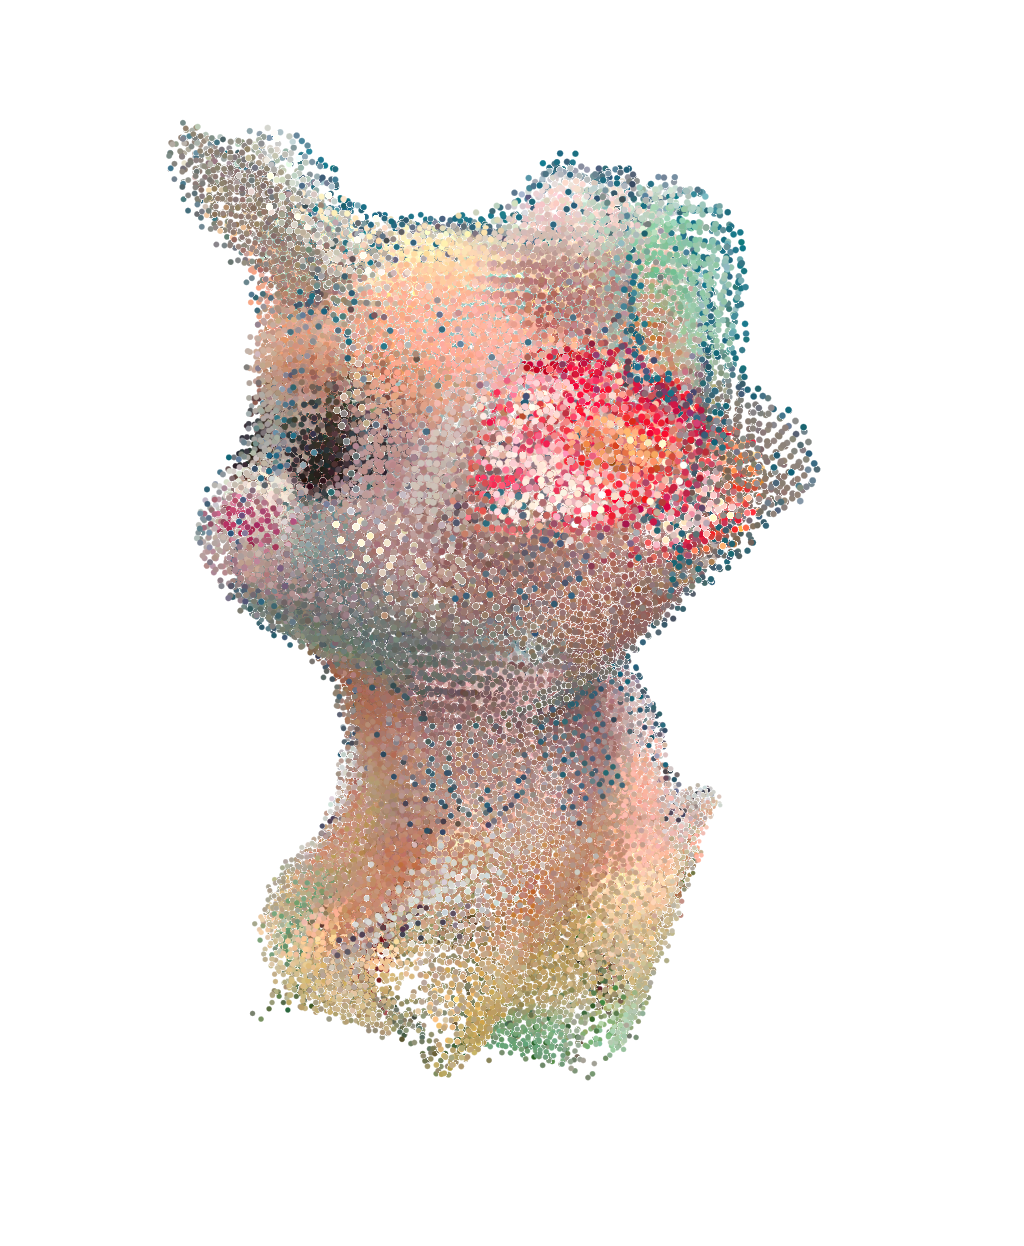
\includegraphics[height=4.5cm]{archivos/experimentacion-3-resultado-nube-2.png}
    \end{subfigure}
    \begin{subfigure}[t]{0.2\textheight}
    	\centering
        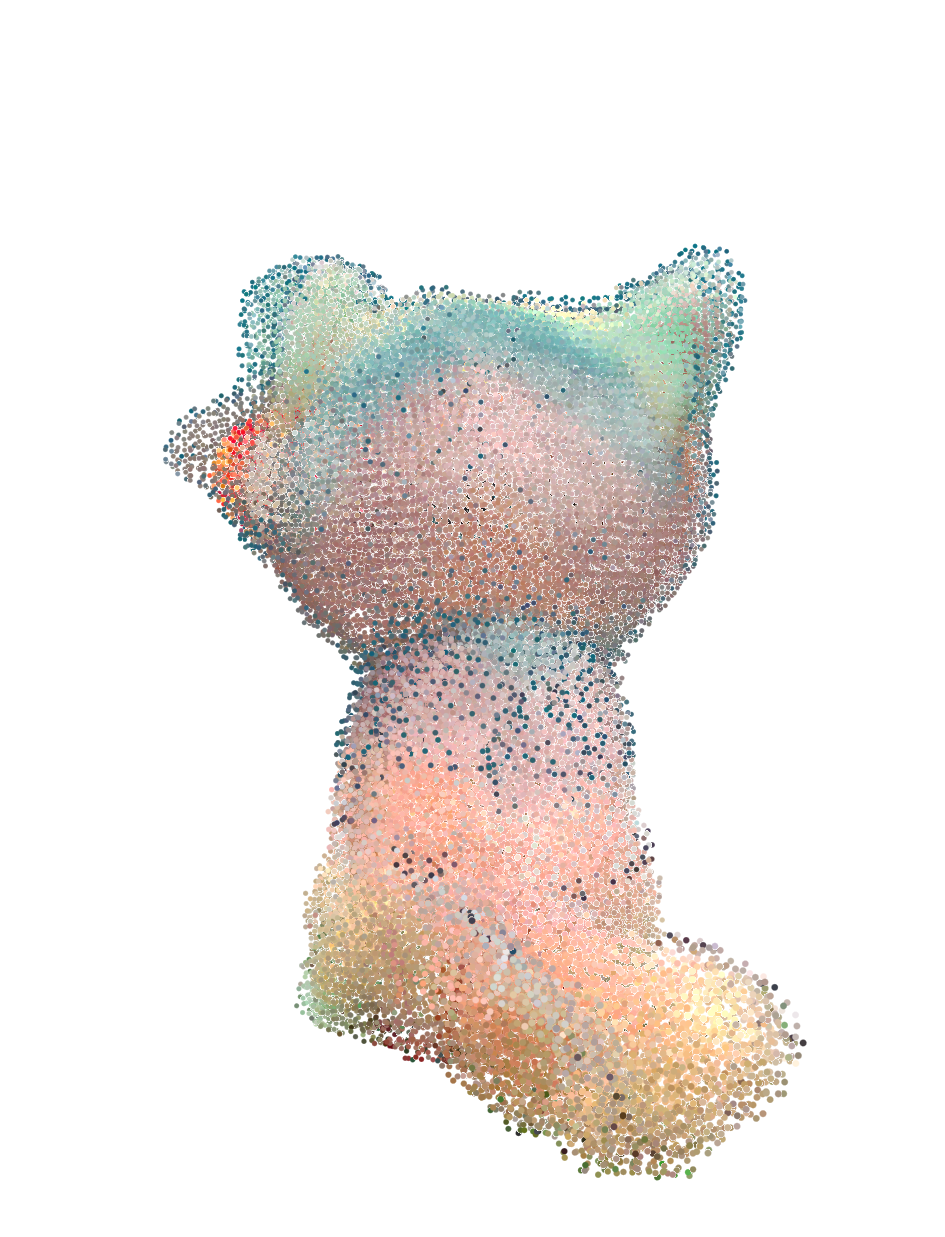
\includegraphics[height=4.5cm]{archivos/experimentacion-3-resultado-nube-3.png}
    \end{subfigure}
    \begin{subfigure}[t]{0.2\textheight}
    	\centering
        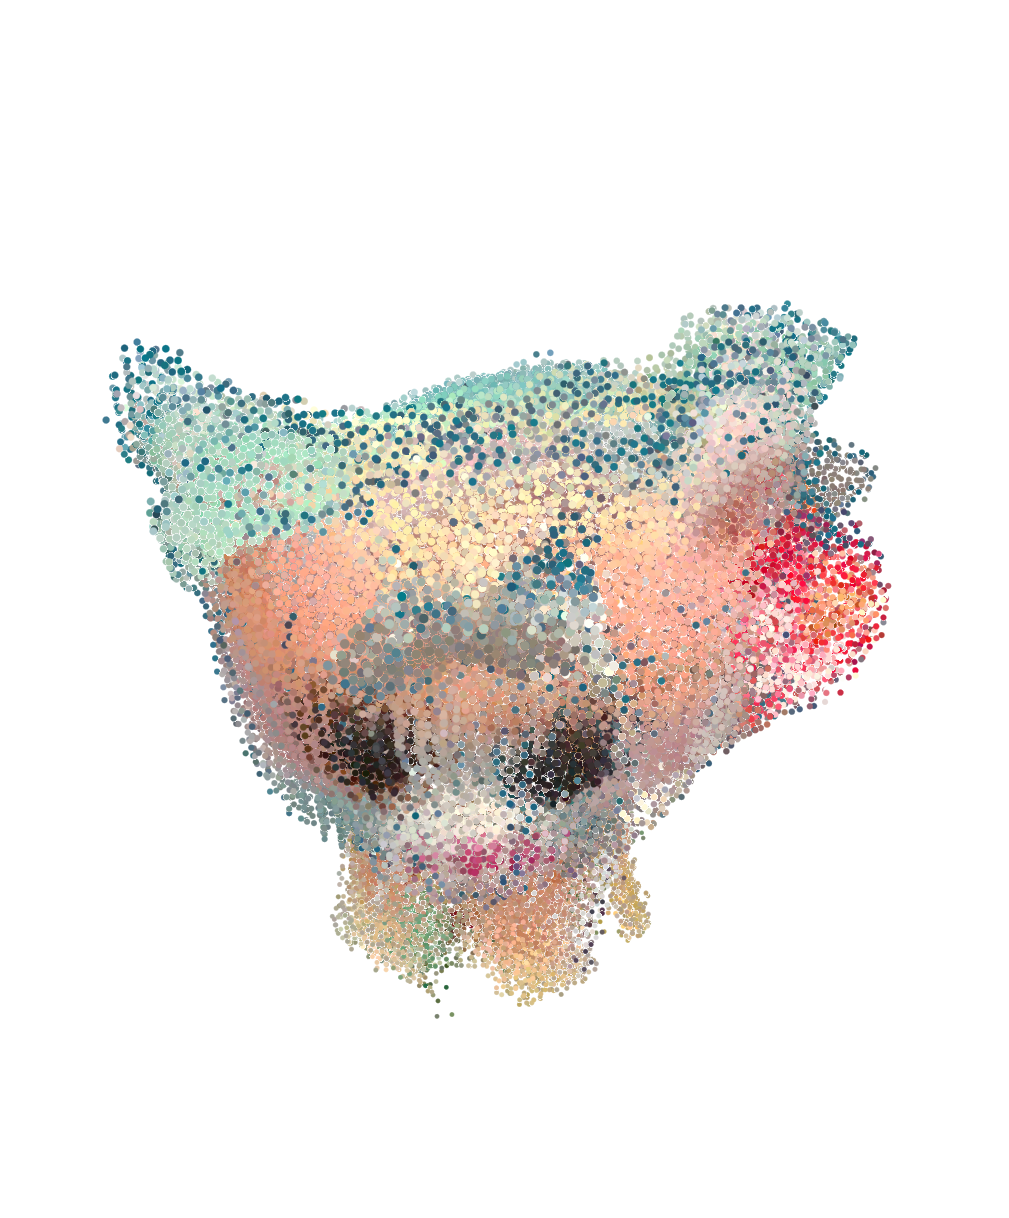
\includegraphics[height=4.5cm]{archivos/experimentacion-3-resultado-nube-4.png}
    \end{subfigure}
    \begin{subfigure}[t]{0.2\textheight}
    	\centering
        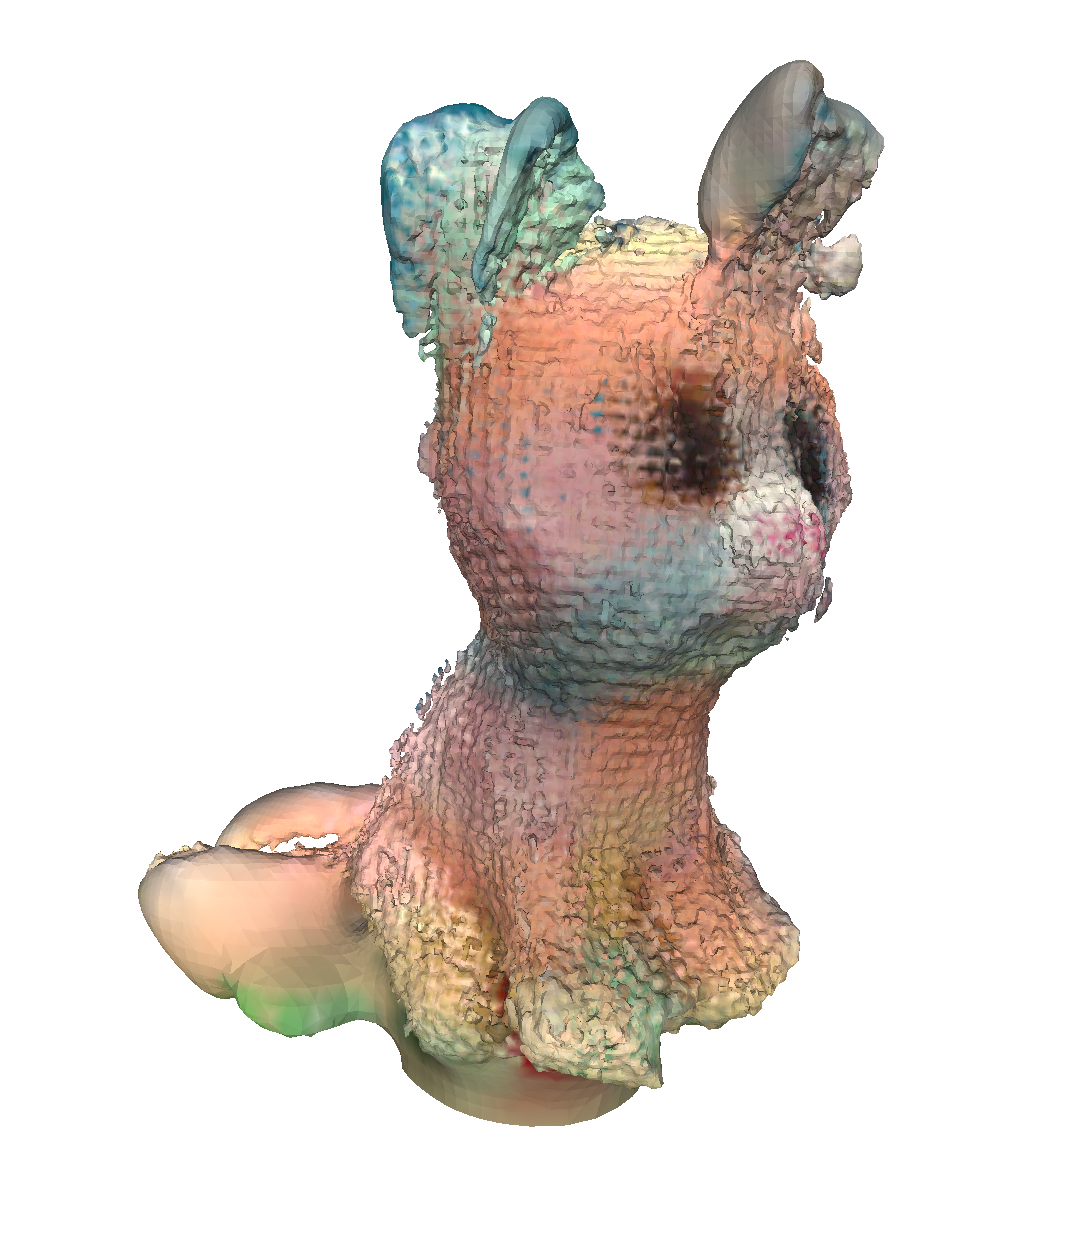
\includegraphics[height=4.5cm]{archivos/experimentacion-3-resultado-malla.png}
    \end{subfigure}
    \begin{subfigure}[t]{0.2\textheight}
    	\centering
        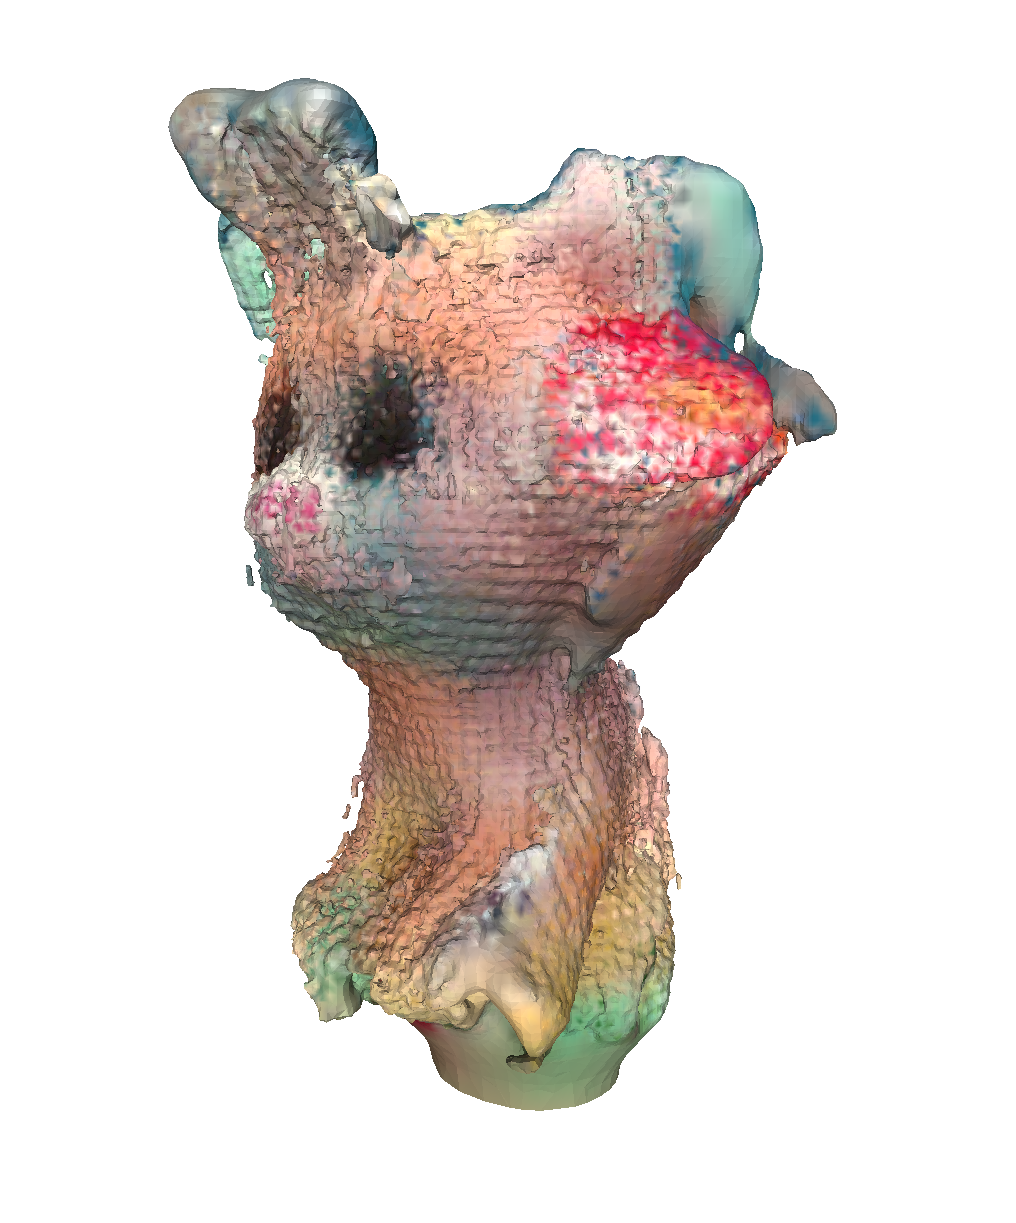
\includegraphics[height=4.5cm]{archivos/experimentacion-3-resultado-malla-2.png}
    \end{subfigure}
    \begin{subfigure}[t]{0.2\textheight}
    	\centering
        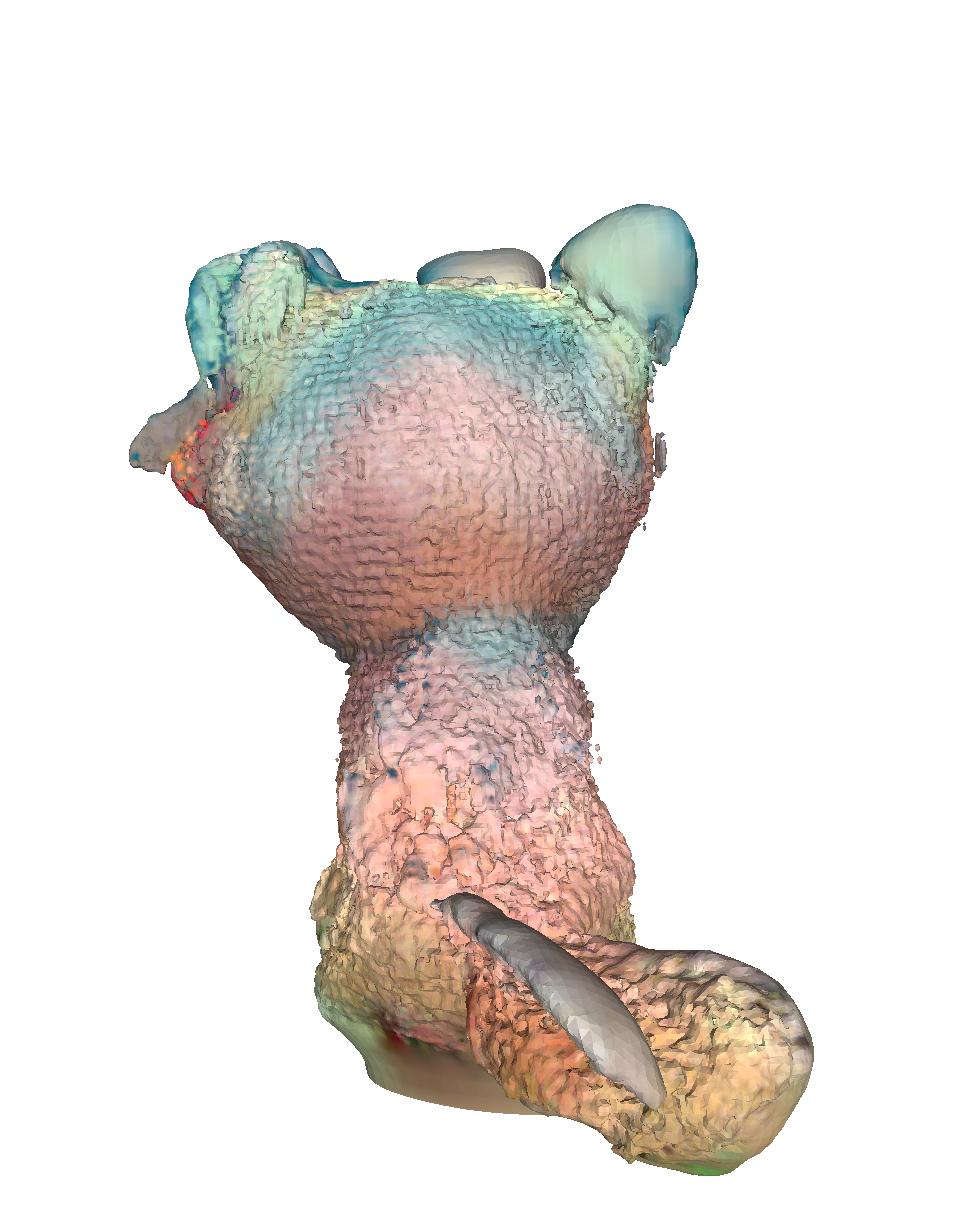
\includegraphics[height=4.5cm]{archivos/experimentacion-3-resultado-malla-3.png}
    \end{subfigure}
    \begin{subfigure}[t]{0.2\textheight}
    	\centering
        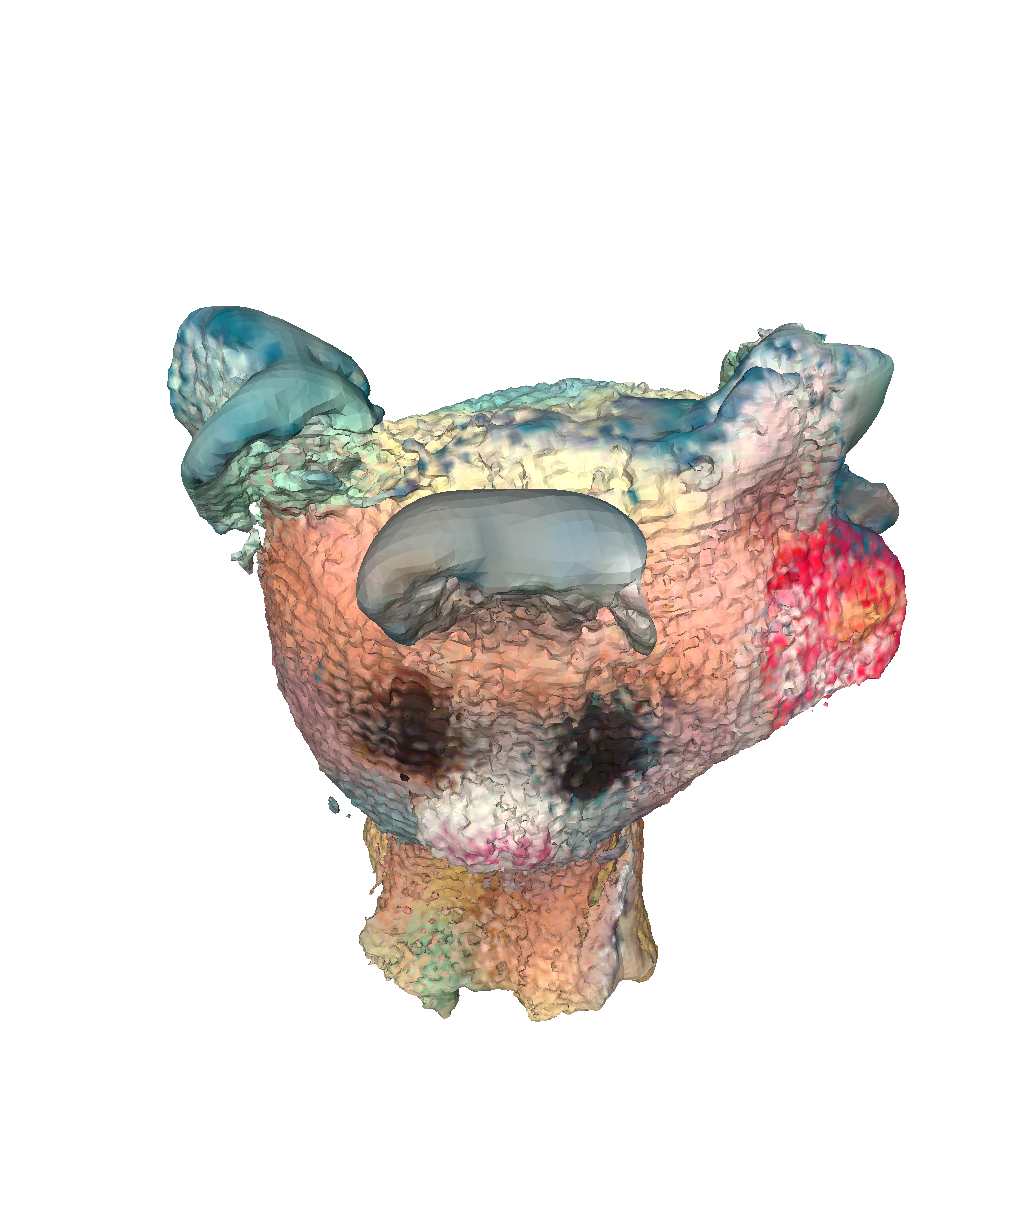
\includegraphics[height=4.5cm]{archivos/experimentacion-3-resultado-malla-4.png}
    \end{subfigure}
    \caption{Resultados de Reconstrucción 3D con objeto usando CUDA-ICP.}
    \label{fig:resultados-reconstruccion-objeto-cuda}
\end{figure}

\begin{table}[h]
    \centering
      \begin{tabular}{rrrrrrrr}
            &       & \multicolumn{2}{c}{Tiempo ICP (s)} & \multicolumn{2}{c}{Tiempo CUDA-ICP (s)} & \multicolumn{2}{c}{Mejora de velocidad} \\
      \multicolumn{1}{l}{Iteración} & \multicolumn{1}{l}{Puntos} & \multicolumn{1}{l}{t/iteracion} & \multicolumn{1}{l}{Total} & \multicolumn{1}{l}{t/iteracion} & \multicolumn{1}{l}{Total} & \multicolumn{1}{l}{\%/iteración} & \multicolumn{1}{l}{Total} \\
      0     & 3540  &       &       &       &       &       &  \\
      1     & 3523  & 1,837 & 1,837 & 0,607 & 0,607 & 302,37\% & 302,37\% \\
      2     & 3497  & 3,056 & 4,892 & 0,977 & 1,585 & 312,62\% & 308,69\% \\
      3     & 3557  & 4,613 & 9,505 & 1,121 & 2,705 & 411,64\% & 351,33\% \\
      4     & 3597  & 3,982 & 13,487 & 0,984 & 3,689 & 404,79\% & 365,59\% \\
      5     & 3710  & 4,133 & 17,620 & 1,159 & 4,849 & 356,47\% & 363,41\% \\
      6     & 3702  & 5,726 & 23,346 & 1,125 & 5,973 & 509,01\% & 390,83\% \\
      7     & 3634  & 3,965 & 27,311 & 1,035 & 7,009 & 382,93\% & 389,66\% \\
      8     & 3755  & 3,877 & 31,188 & 1,051 & 8,060 & 368,94\% & 386,96\% \\
      9     & 3686  & 4,259 & 35,446 & 1,305 & 9,365 & 326,30\% & 378,50\% \\
      10    & 3792  & 3,364 & 38,811 & 1,012 & 10,377 & 332,35\% & 374,00\% \\
      11    & 3775  & 3,536 & 42,347 & 1,315 & 11,693 & 268,81\% & 362,17\% \\
      12    & 3883  & 3,586 & 45,933 & 0,971 & 12,663 & 369,47\% & 362,73\% \\
      13    & 3855  & 3,746 & 49,678 & 1,163 & 13,827 & 321,95\% & 359,30\% \\
      14    & 3842  & 7,131 & 56,809 & 1,375 & 15,201 & 518,65\% & 373,71\% \\
      15    & 3994  & 5,695 & 62,504 & 1,217 & 16,419 & 467,87\% & 380,69\% \\
      16    & 4127  & 6,641 & 69,145 & 1,292 & 17,711 & 514,04\% & 390,42\% \\
      17    & 4443  & 6,107 & 75,252 & 1,198 & 18,909 & 509,77\% & 397,98\% \\
      18    & 4268  & 4,798 & 80,050 & 1,621 & 20,530 & 295,94\% & 389,92\% \\
      19    & 4128  & 5,402 & 85,451 & 1,464 & 21,993 & 369,04\% & 388,53\% \\
      20    & 3955  & 5,822 & 91,273 & 1,315 & 23,309 & 442,66\% & 391,59\% \\
      21    & 3931  & 4,329 & 95,602 & 1,262 & 24,570 & 343,10\% & 389,10\% \\
      22    & 4000  & 5,393 & 100,995 & 1,587 & 26,157 & 339,94\% & 386,11\% \\
      23    & 3922  & 6,951 & 107,947 & 1,553 & 27,710 & 447,57\% & 389,56\% \\
      24    & 3828  & 5,326 & 113,272 & 1,621 & 29,331 & 328,51\% & 386,18\% \\
      25    & 3739  & 6,527 & 119,799 & 1,574 & 30,905 & 414,58\% & 387,63\% \\
      26    & 3687  & 5,665 & 125,464 & 1,531 & 32,436 & 370,08\% & 386,80\% \\
      27    & 3665  & 7,183 & 132,647 & 1,810 & 34,246 & 396,91\% & 387,34\% \\
      28    & 3658  & 8,995 & 141,642 & 1,468 & 35,714 & 612,74\% & 396,60\% \\
      29    & 3746  & 6,553 & 148,195 & 1,497 & 37,211 & 437,62\% & 398,25\% \\
      30    & 3747  & 8,390 & 156,585 & 1,774 & 38,985 & 473,00\% & 401,65\% \\
      31    & 3632  & 9,176 & 165,761 & 1,908 & 40,893 & 480,98\% & 405,35\% \\
      32    & 3516  & 8,287 & 174,048 & 1,726 & 42,619 & 480,13\% & 408,38\% \\
      33    & 3497  & 5,666 & 179,714 & 1,971 & 44,590 & 287,51\% & 403,04\% \\
      34    & 3513  & 5,748 & 185,462 & 1,948 & 46,538 & 295,03\% & 398,52\% \\
      35    & 3522  & 5,483 & 190,945 & 1,837 & 48,375 & 298,48\% & 394,72\% \\
      36    & 3558  & 5,042 & 195,986 & 1,798 & 50,173 & 280,45\% & 390,62\% \\
      37    & 3613  & 5,722 & 201,708 & 1,961 & 52,134 & 291,73\% & 386,90\% \\
      38    & 3678  & 5,355 & 207,063 & 1,835 & 53,969 & 291,74\% & 383,67\% \\
      39    & 3693  & 8,961 & 216,024 & 1,999 & 55,969 & 448,18\% & 385,97\% \\
      40    & 3638  & 6,771 & 222,795 & 1,999 & 57,967 & 338,78\% & 384,34\% \\
      41    & 3662  & 8,201 & 230,996 & 1,928 & 59,896 & 425,32\% & 385,66\% \\
    \end{tabular}%
    \caption{Resultados de Reconstrucción 3D con objeto.}
    \label{tab:resultado-objeto}%
\end{table}%
  

\section{Resultados de la reconstrucción completa de un cuerpo humano}

Para lograr un buen resultado en la reconstrucción del cuerpo humano se ha realizado la fase de adquisición con el sujeto sentado en una silla de oficina, de esta forma el sujeto puede rotar cómodamente 360º intentando mantener su cuerpo rígido de forma que la reconstrucción sea más limpia.
En esta fase de adquisición se han realizado 30 capturas al sujeto, que es lo que ha tardado en rotar 360º con una frecuencia de capturación de 1 imágen por cada 0.5 segundos.

Para el algoritmo \gls{icp} se ha establecido un máximo de 200 iteraciones y el límite máximo de distancia entre correspondencias se ha subido a 0.5m debido a que el cuerpo a escanear es mucho más grande y se mueve a una velocidad que no es constante como sí lo hacía el objeto encima del plato giratorio, por lo que es posible que alguna distancia pueda llegar a medir más.

De nuevo, en las figuras \ref{fig:resultados-reconstruccion-cuerpo-icp} y \ref{fig:resultados-reconstruccion-cuerpo-cuda} podemos ver los resultados de la reconstrucción expresados de la misma forma que el objeto, es decir, las primeras cuatro imágenes en nubes de puntos, y las siguientes cuatro con una malla generada a partir de los puntos.

Si analizamos la Tabla \ref{tab:resultado-cuerpo}, podemos ver que los resultados son parecido al del objeto, con unos tiempos en general más grandes debido a que la cantidad de puntos de cada escena es mucho mayor comparado con las escenas del objeto.
Aunque el algoritmo con \gls{cuda} vuelve a ser mucho más rápido, volvemos a tener el problema de que el resultado no es tan correcto como lo es en \gls{icp} de \gls{pcl}.
Este es un problema que tenemos con la librería de \gls{cuda} ya que no permite mucha configuración a la hora de lanzar el algoritmo, como si lo hace \gls{pcl}, y no se ha podido corregir el error.

\begin{figure}[h]
    \centering
    \begin{subfigure}[t]{0.2\textheight}
    	\centering
        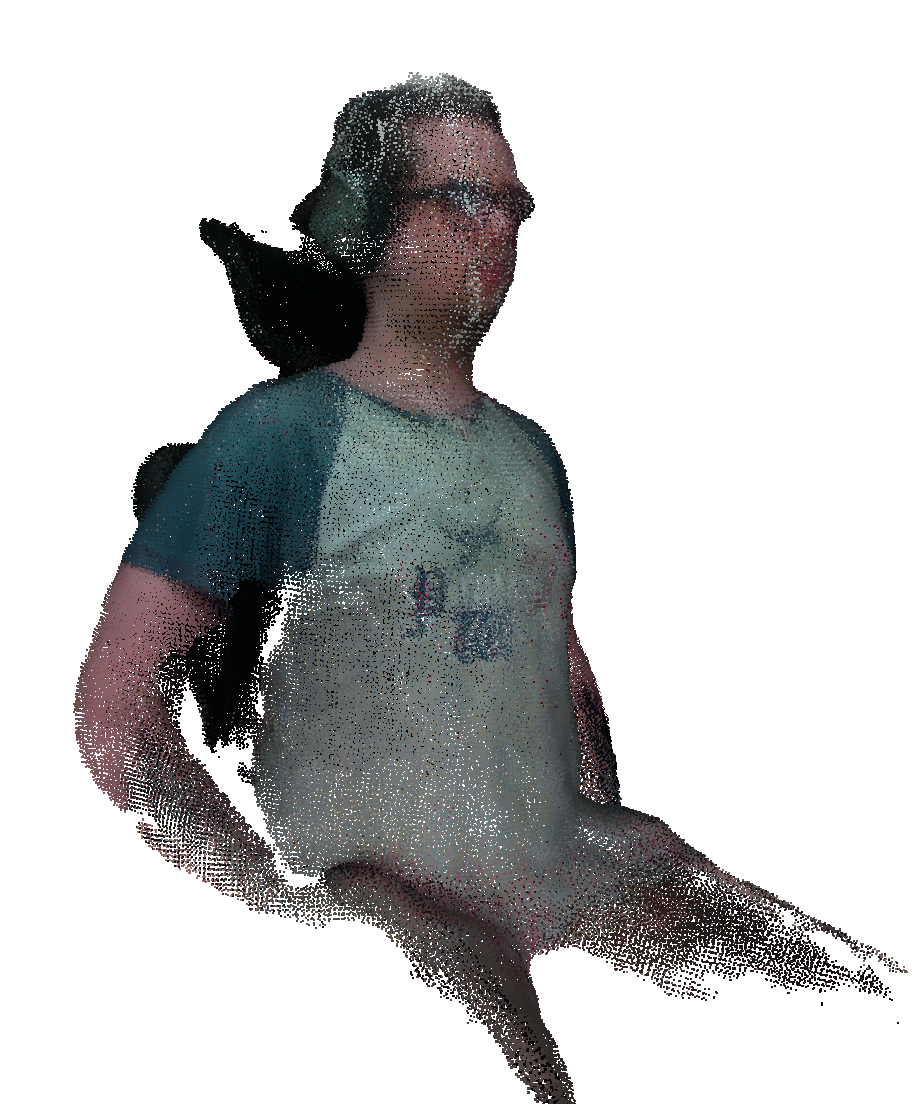
\includegraphics[height=4.5cm]{archivos/experimentacion-4-resultado-nube.png}
    \end{subfigure}
    \begin{subfigure}[t]{0.2\textheight}
    	\centering
        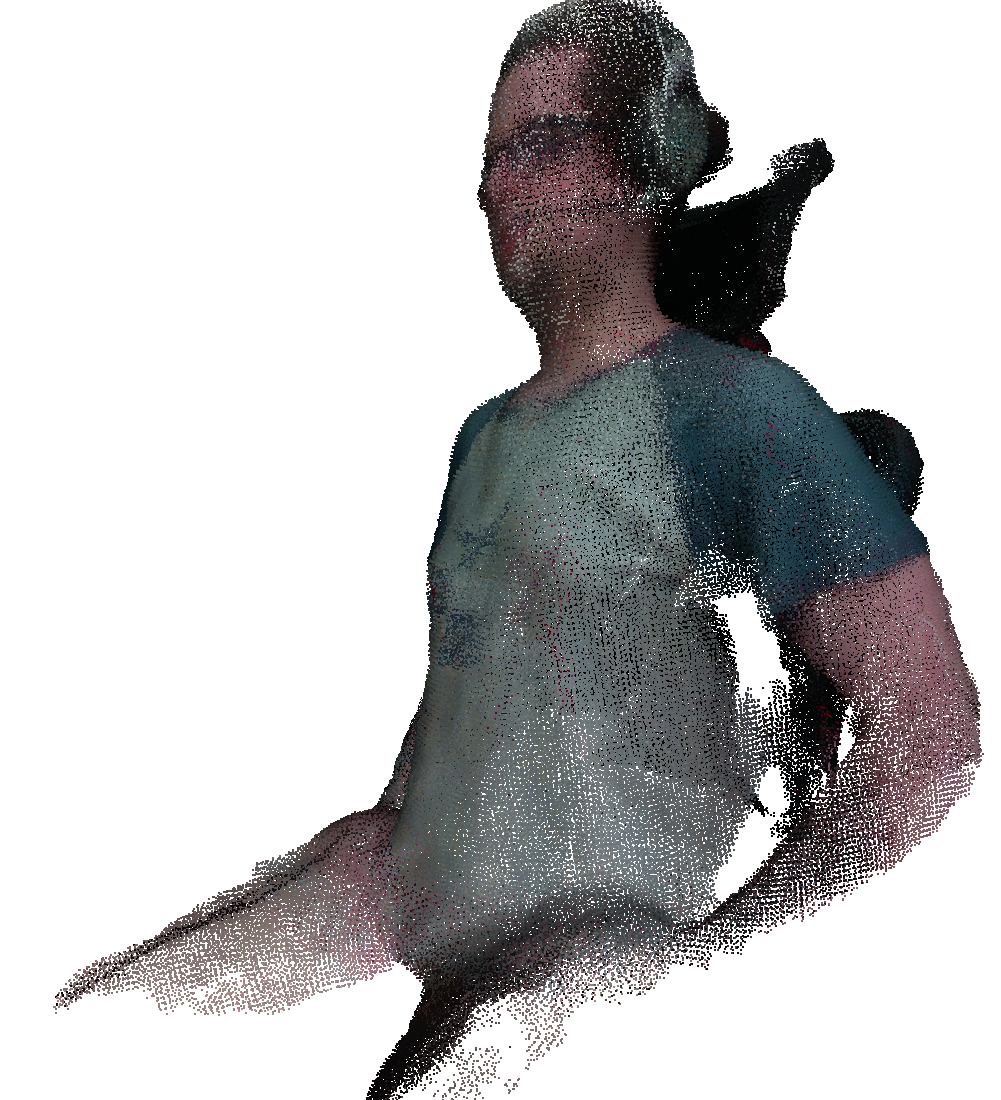
\includegraphics[height=4.5cm]{archivos/experimentacion-4-resultado-nube-2.png}
    \end{subfigure}
    \begin{subfigure}[t]{0.2\textheight}
    	\centering
        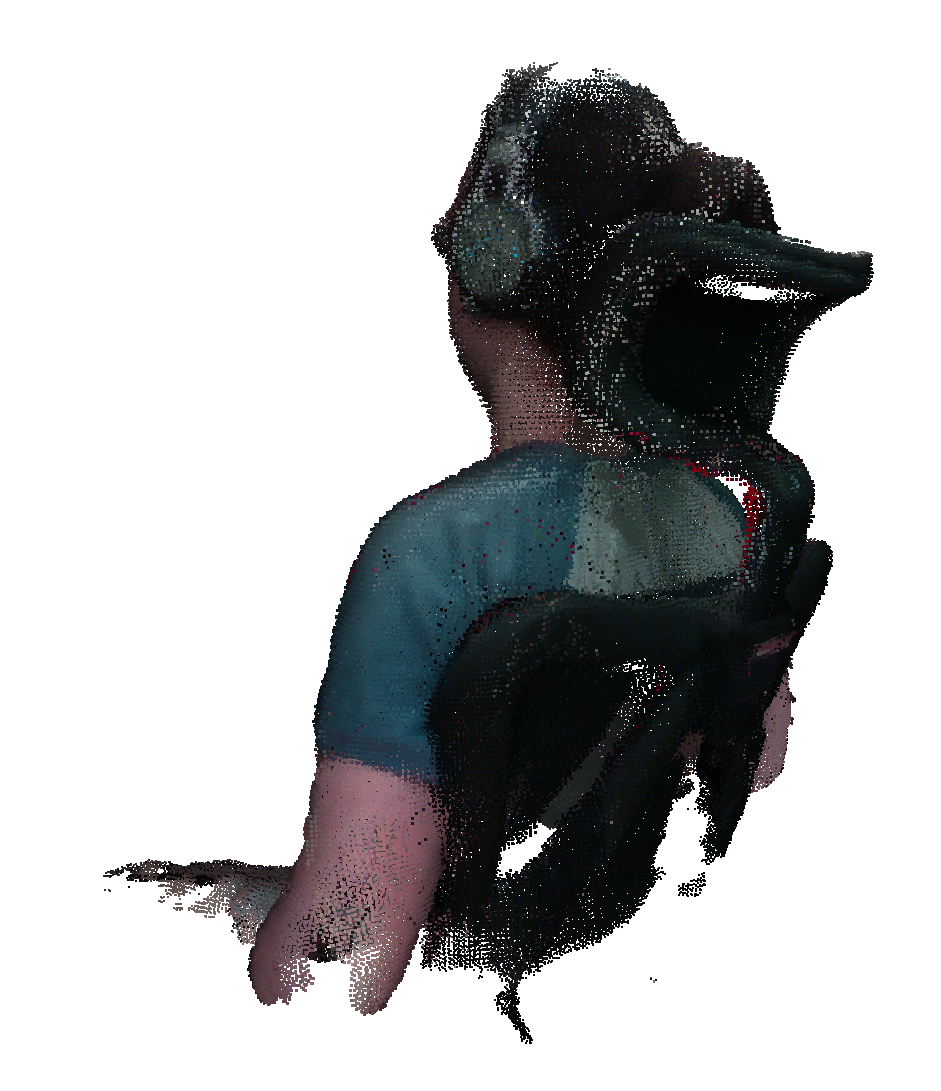
\includegraphics[height=4.5cm]{archivos/experimentacion-4-resultado-nube-3.png}
    \end{subfigure}
    \begin{subfigure}[t]{0.2\textheight}
    	\centering
        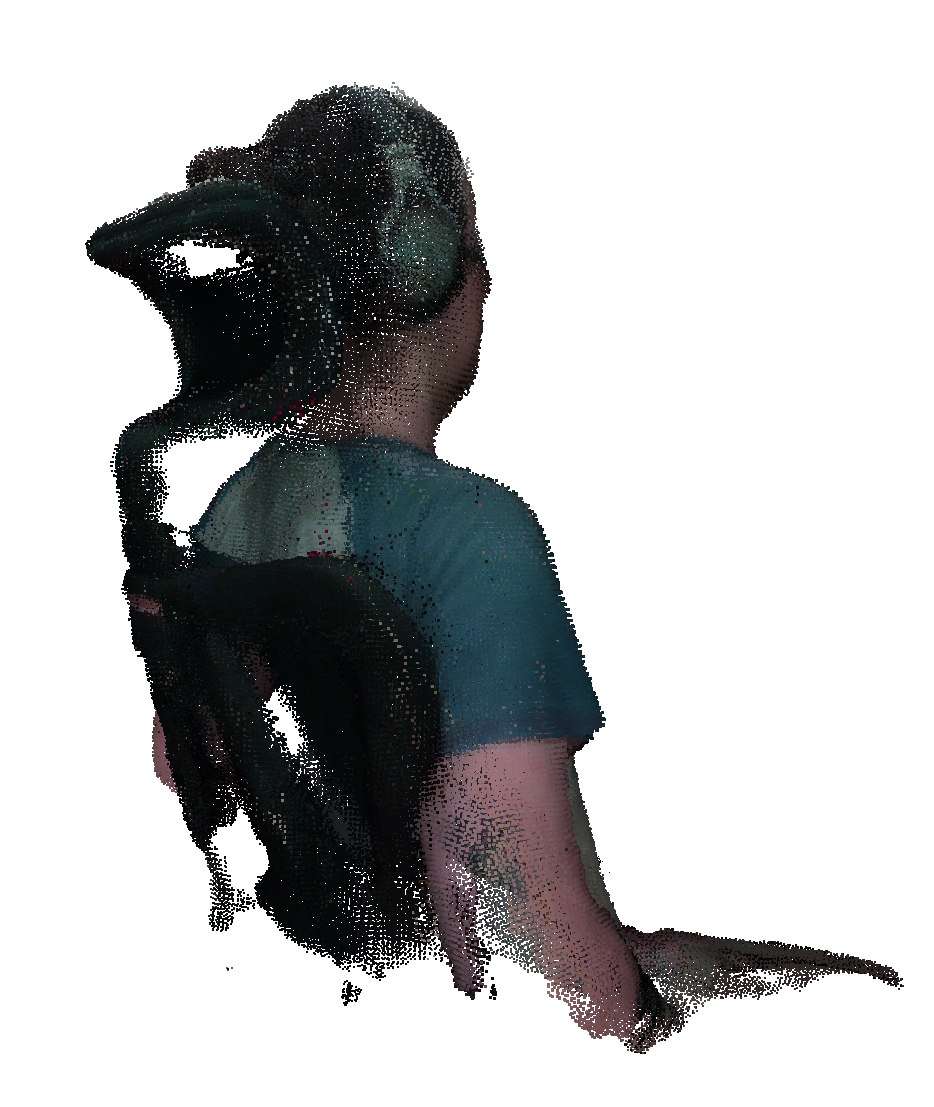
\includegraphics[height=4.5cm]{archivos/experimentacion-4-resultado-nube-4.png}
    \end{subfigure}
    \begin{subfigure}[t]{0.2\textheight}
    	\centering
        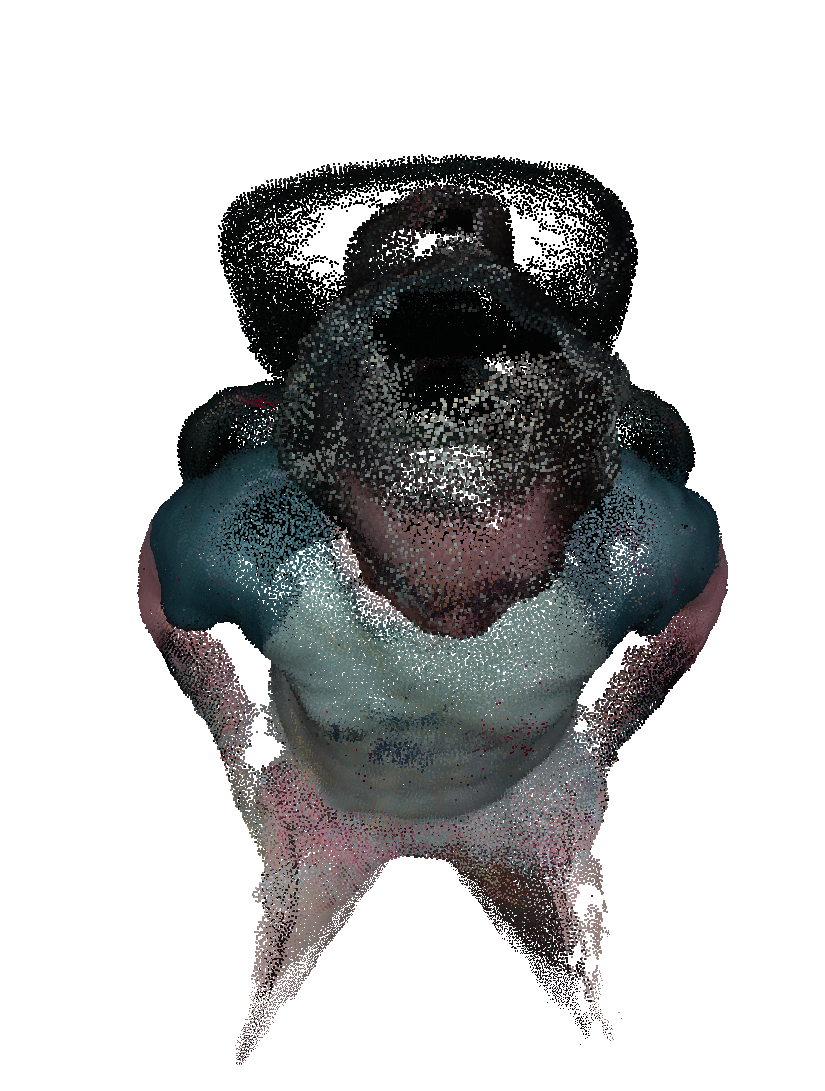
\includegraphics[height=4.5cm]{archivos/experimentacion-4-resultado-nube-5.png}
    \end{subfigure}
    \begin{subfigure}[t]{0.2\textheight}
    	\centering
        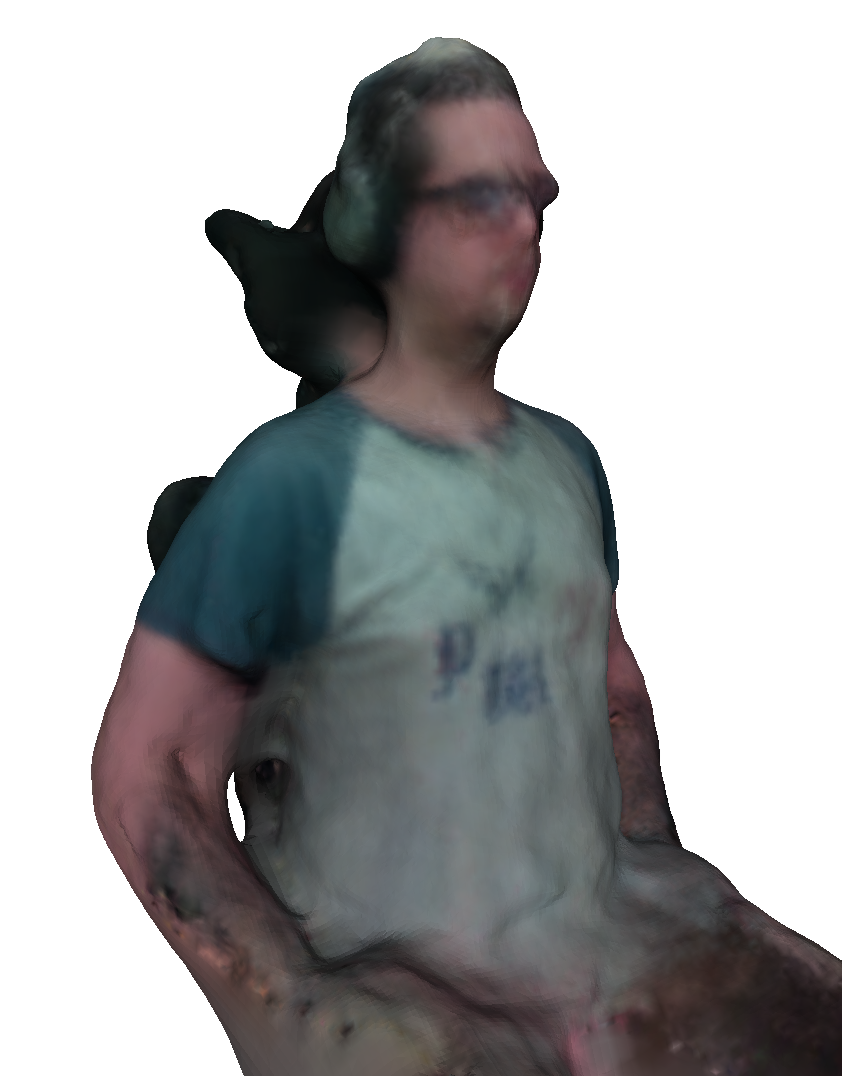
\includegraphics[height=4.5cm]{archivos/experimentacion-4-resultado-malla.png}
    \end{subfigure}
    \begin{subfigure}[t]{0.2\textheight}
    	\centering
        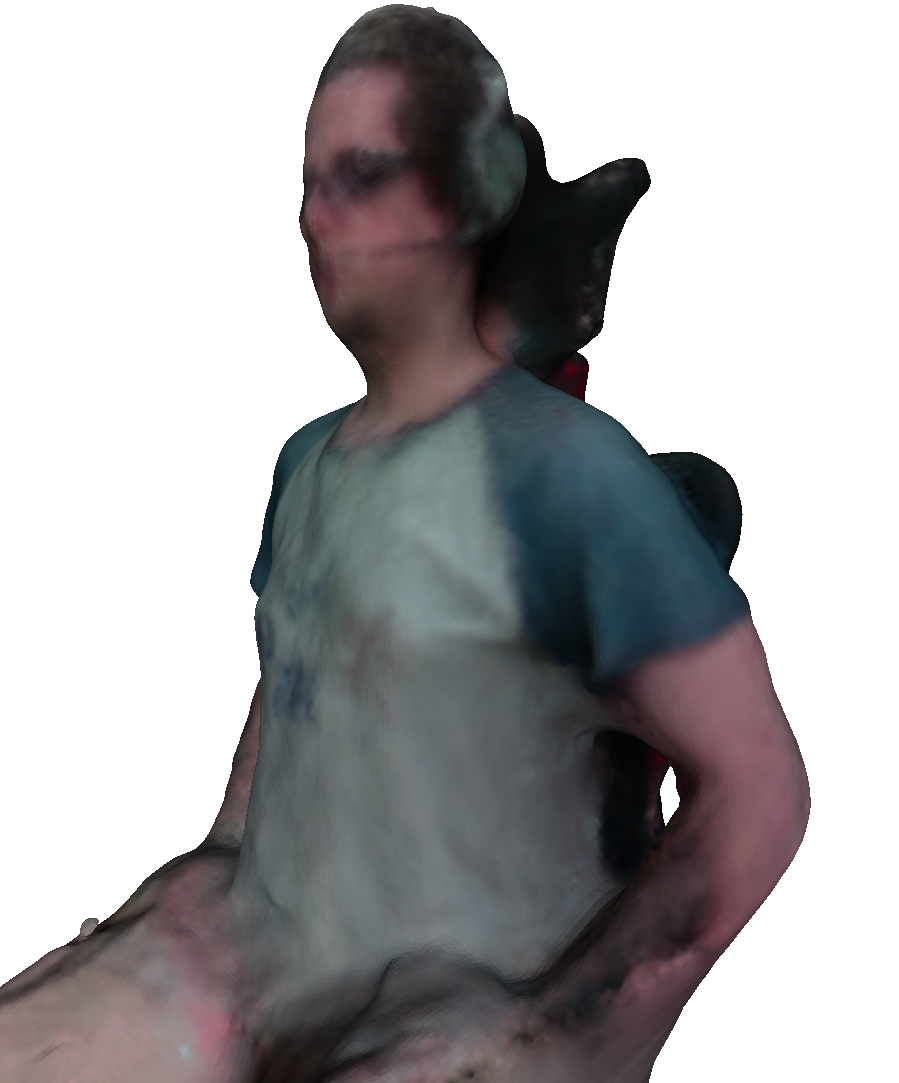
\includegraphics[height=4.5cm]{archivos/experimentacion-4-resultado-malla-2.png}
    \end{subfigure}
    \begin{subfigure}[t]{0.2\textheight}
    	\centering
        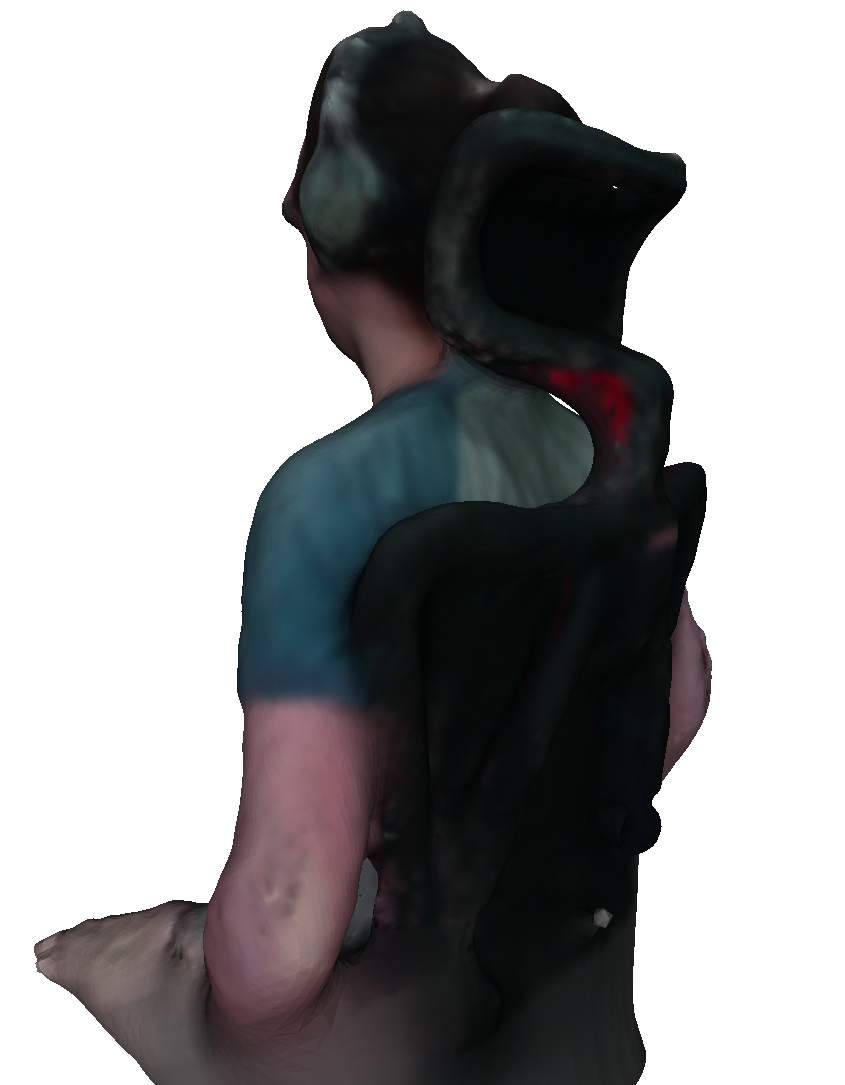
\includegraphics[height=4.5cm]{archivos/experimentacion-4-resultado-malla-3.png}
    \end{subfigure}
    \begin{subfigure}[t]{0.2\textheight}
    	\centering
        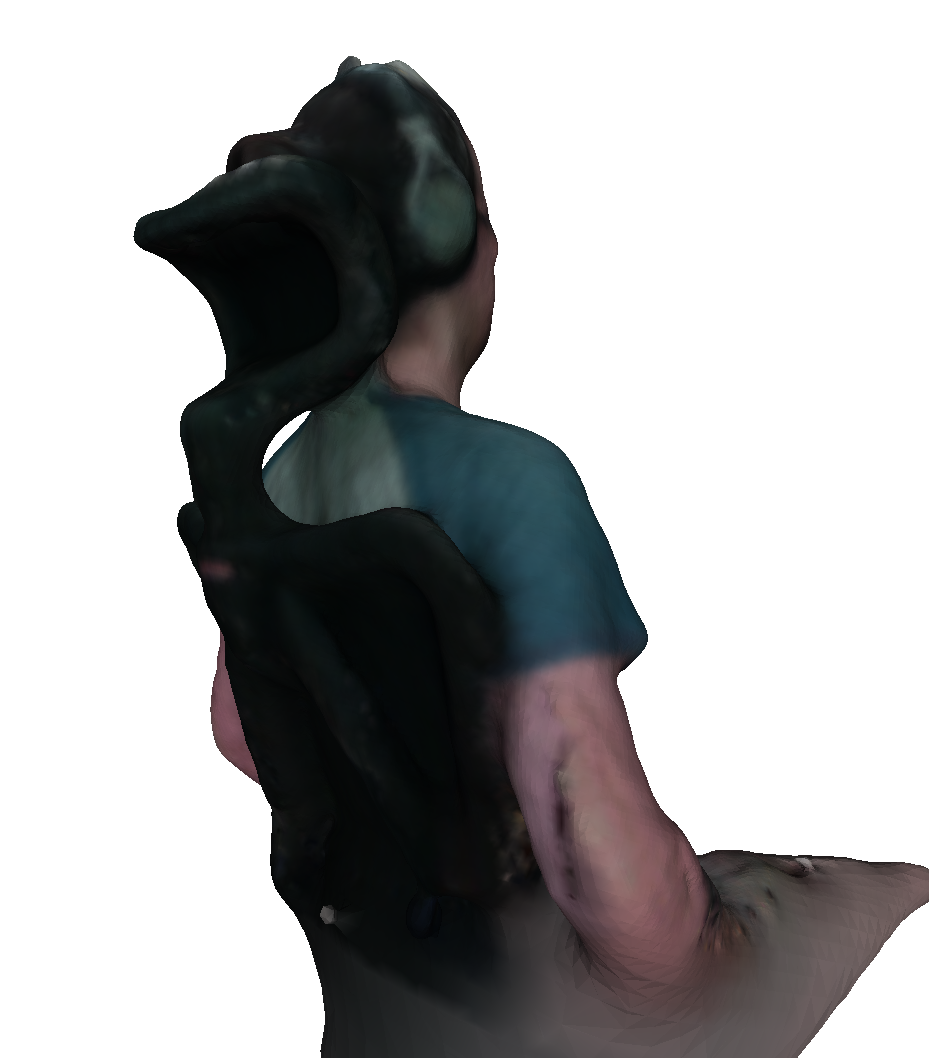
\includegraphics[height=4.5cm]{archivos/experimentacion-4-resultado-malla-4.png}
    \end{subfigure}
    \begin{subfigure}[t]{0.2\textheight}
    	\centering
        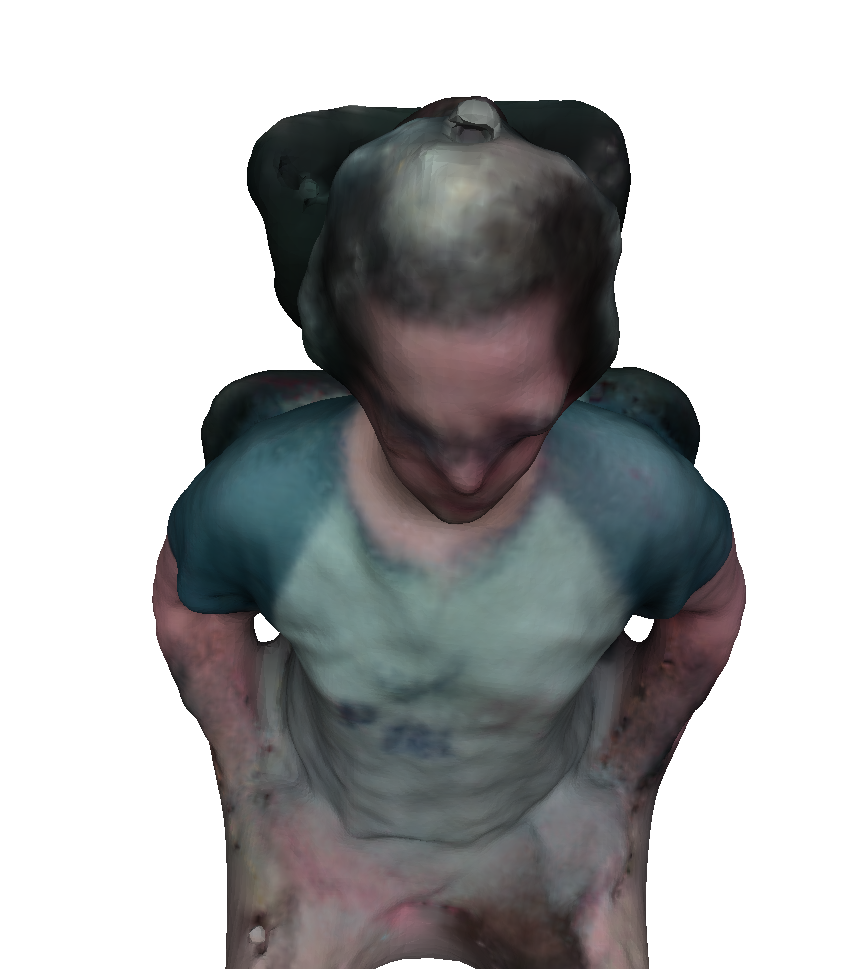
\includegraphics[height=4.5cm]{archivos/experimentacion-4-resultado-malla-5.png}
    \end{subfigure}
    \caption{Resultados de Reconstrucción 3D de un cuerpo humano usando ICP.}
    \label{fig:resultados-reconstruccion-cuerpo-icp}
\end{figure}

\begin{figure}[h]
    \centering
    \begin{subfigure}[t]{0.2\textheight}
    	\centering
        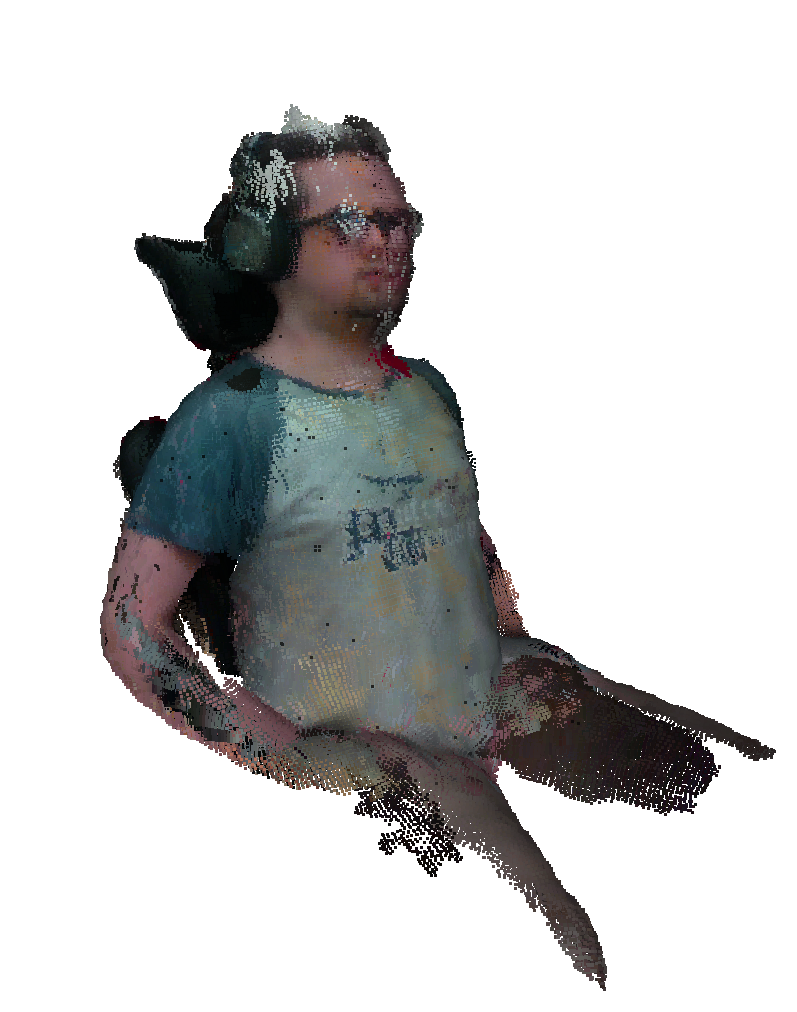
\includegraphics[height=4.5cm]{archivos/experimentacion-5-resultado-nube.png}
    \end{subfigure}
    \begin{subfigure}[t]{0.2\textheight}
    	\centering
        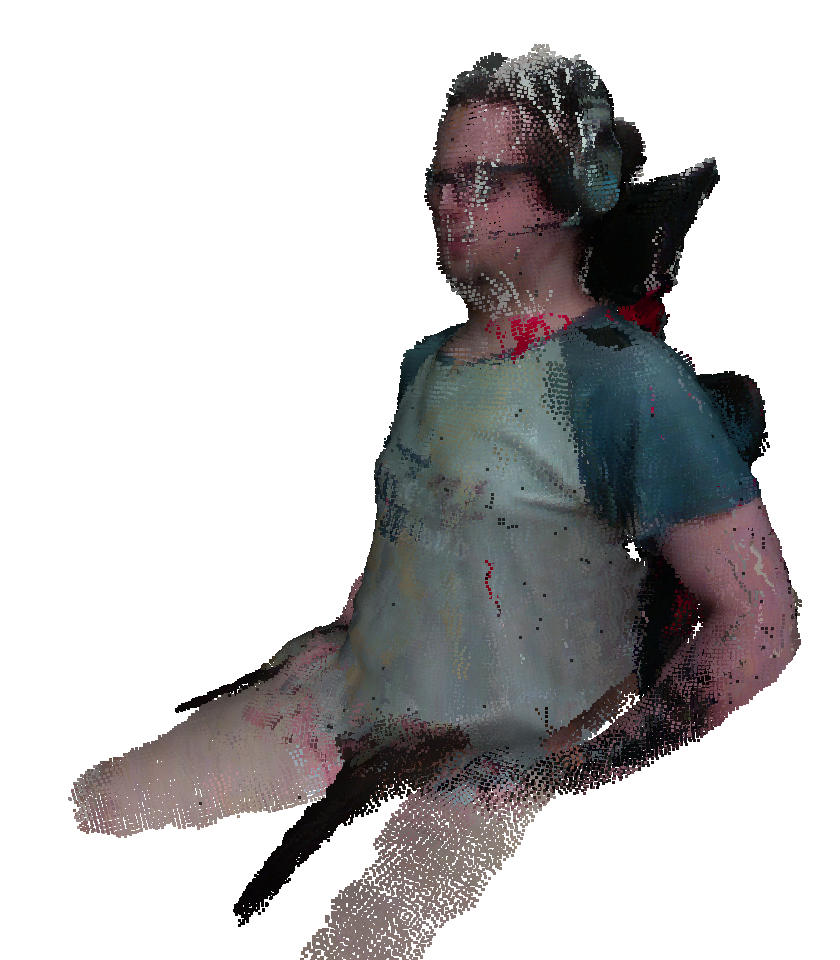
\includegraphics[height=4.5cm]{archivos/experimentacion-5-resultado-nube-2.png}
    \end{subfigure}
    \begin{subfigure}[t]{0.2\textheight}
    	\centering
        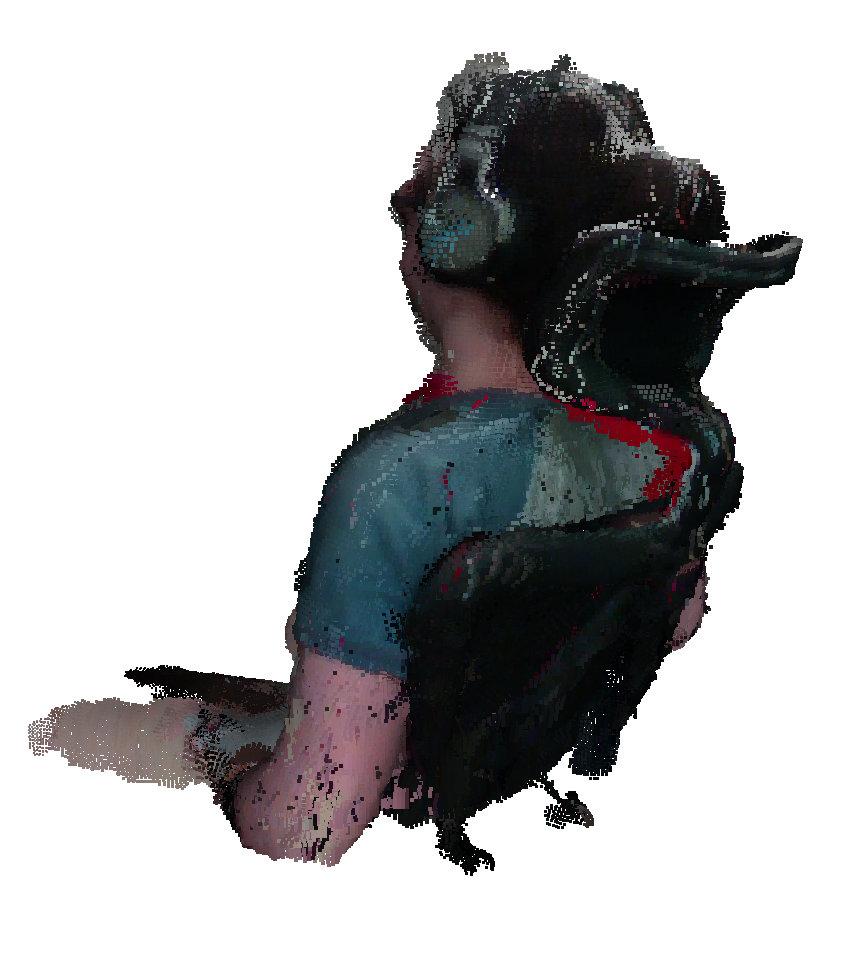
\includegraphics[height=4.5cm]{archivos/experimentacion-5-resultado-nube-3.png}
    \end{subfigure}
    \begin{subfigure}[t]{0.2\textheight}
    	\centering
        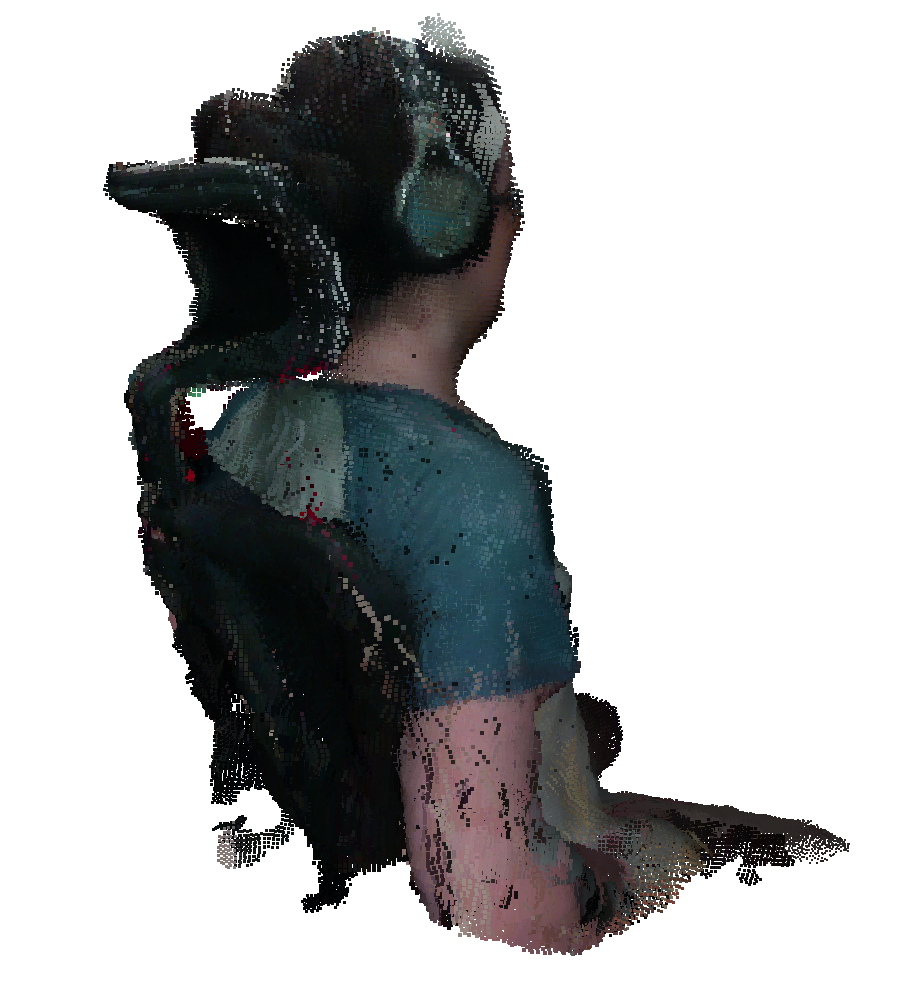
\includegraphics[height=4.5cm]{archivos/experimentacion-5-resultado-nube-4.png}
    \end{subfigure}
    \begin{subfigure}[t]{0.2\textheight}
    	\centering
        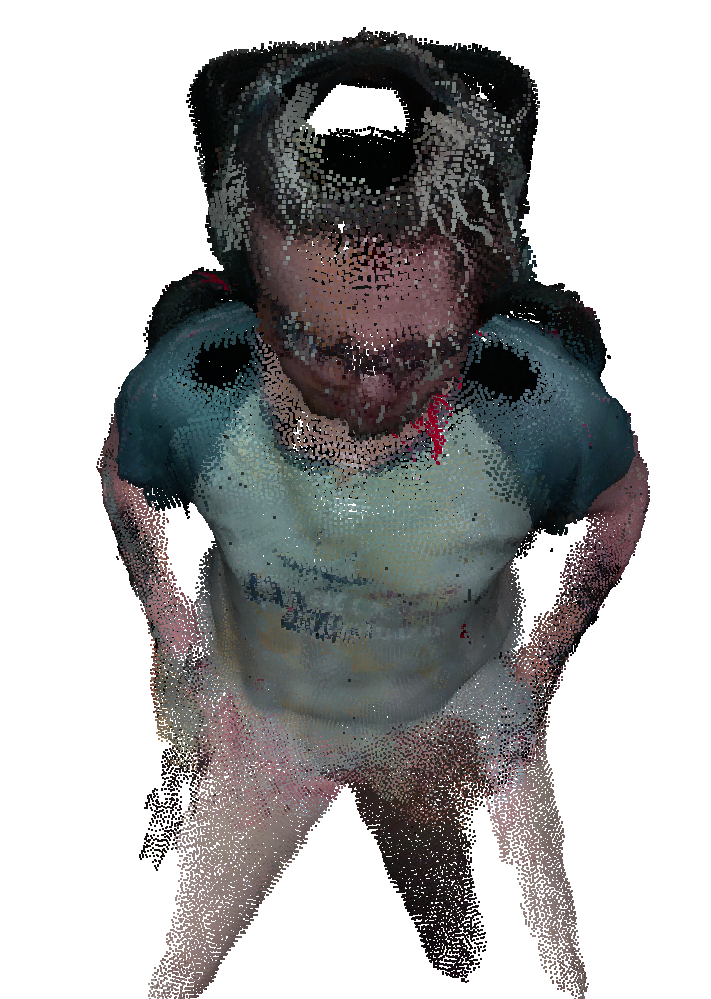
\includegraphics[height=4.5cm]{archivos/experimentacion-5-resultado-nube-5.png}
    \end{subfigure}
    \begin{subfigure}[t]{0.2\textheight}
    	\centering
        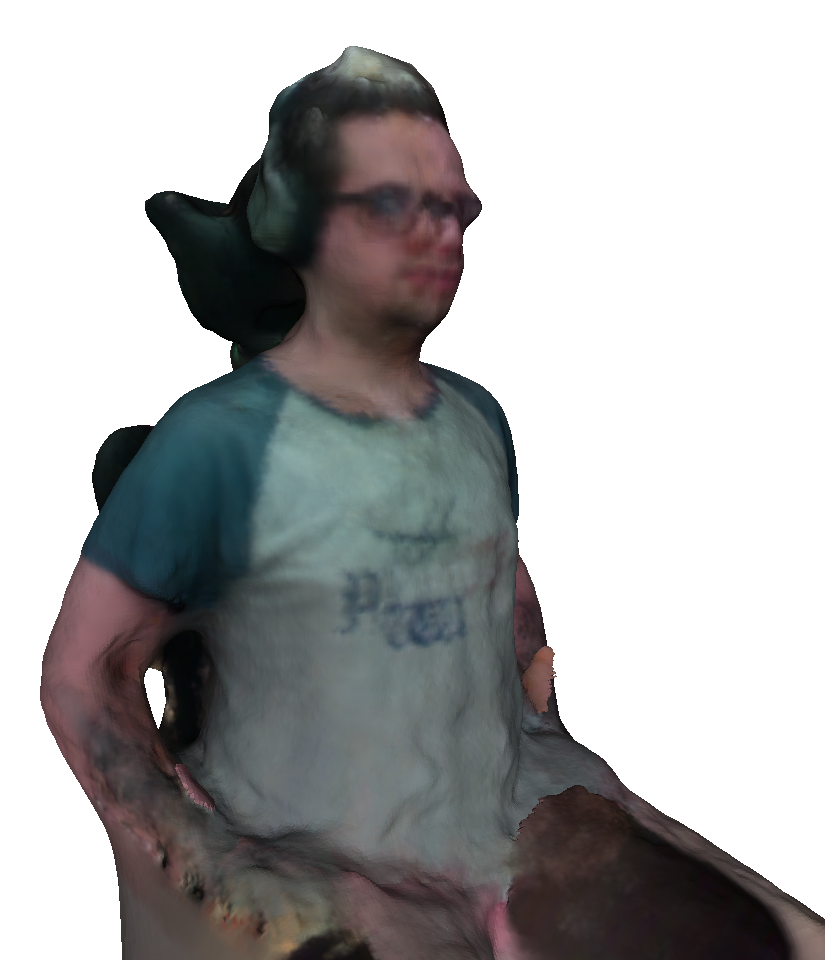
\includegraphics[height=4.5cm]{archivos/experimentacion-5-resultado-malla.png}
    \end{subfigure}
    \begin{subfigure}[t]{0.2\textheight}
    	\centering
        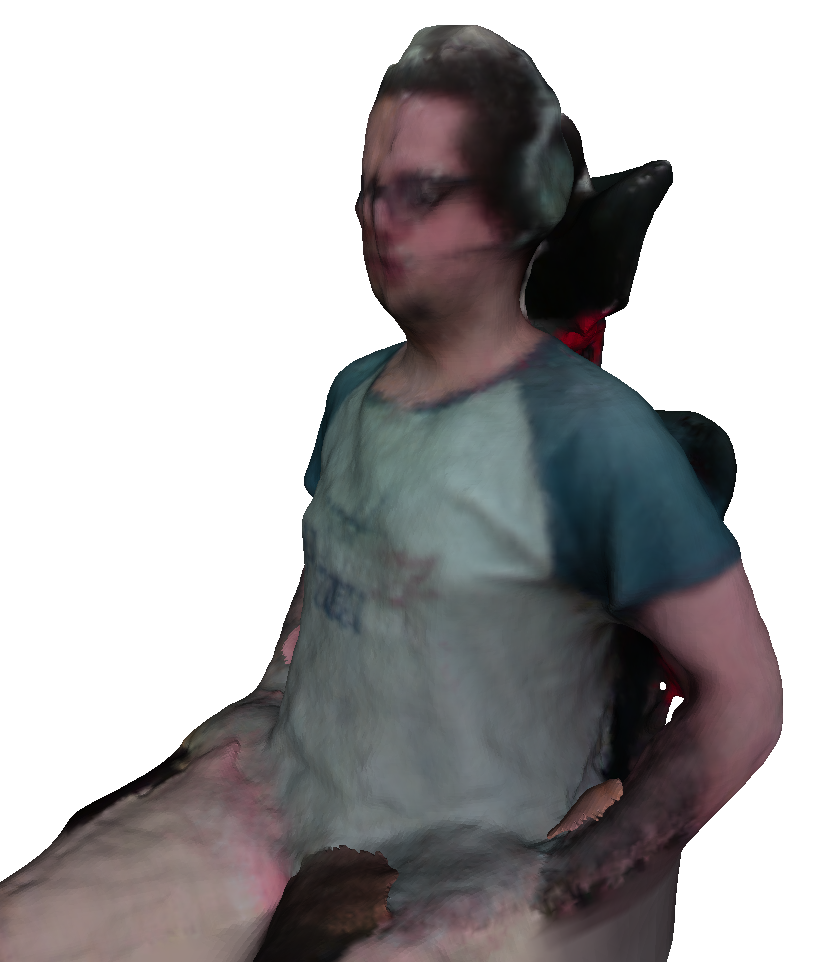
\includegraphics[height=4.5cm]{archivos/experimentacion-5-resultado-malla-2.png}
    \end{subfigure}
    \begin{subfigure}[t]{0.2\textheight}
    	\centering
        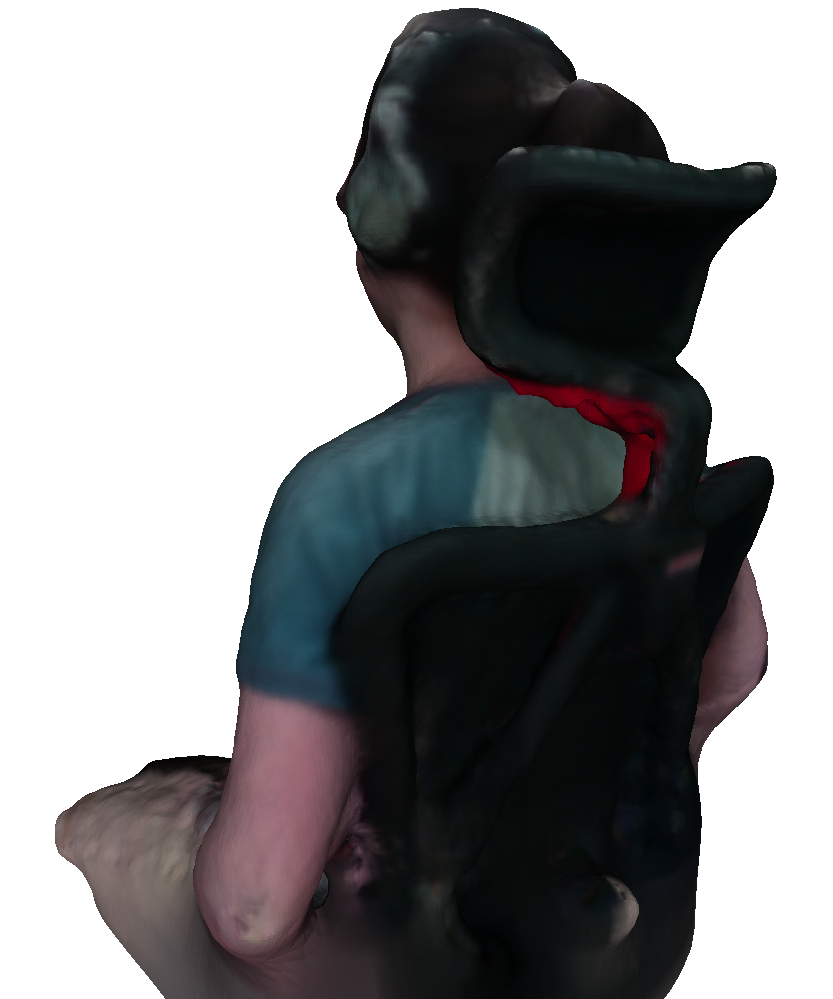
\includegraphics[height=4.5cm]{archivos/experimentacion-5-resultado-malla-3.png}
    \end{subfigure}
    \begin{subfigure}[t]{0.2\textheight}
    	\centering
        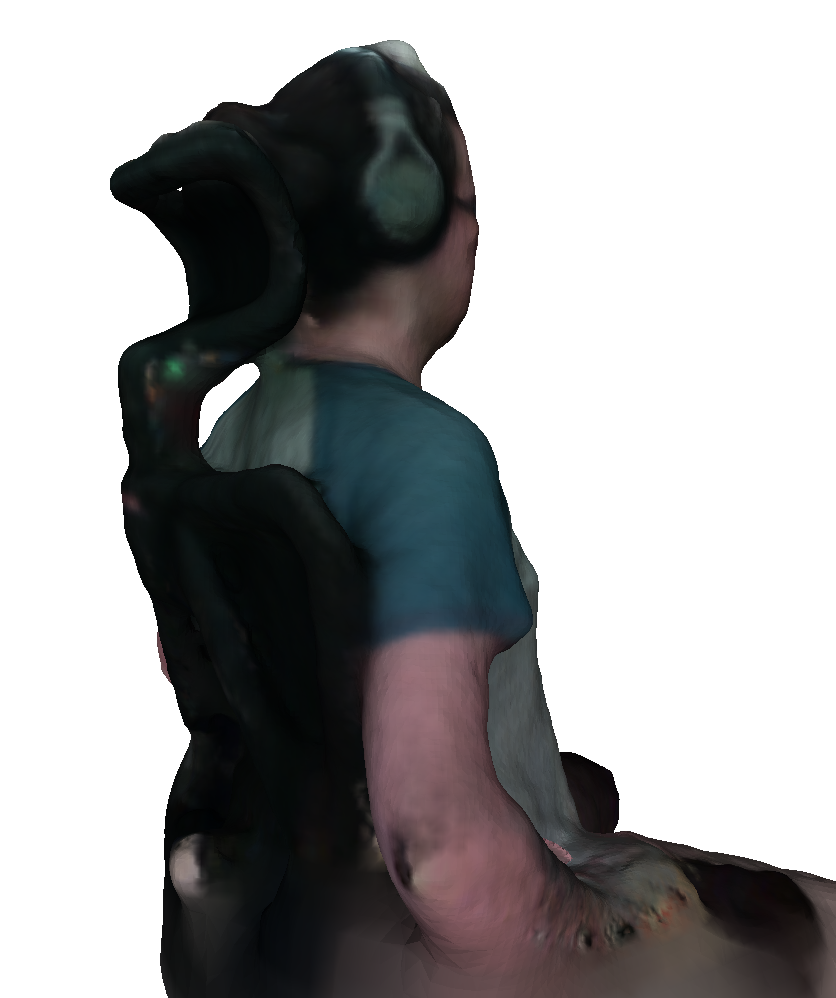
\includegraphics[height=4.5cm]{archivos/experimentacion-5-resultado-malla-4.png}
    \end{subfigure}
    \begin{subfigure}[t]{0.2\textheight}
    	\centering
        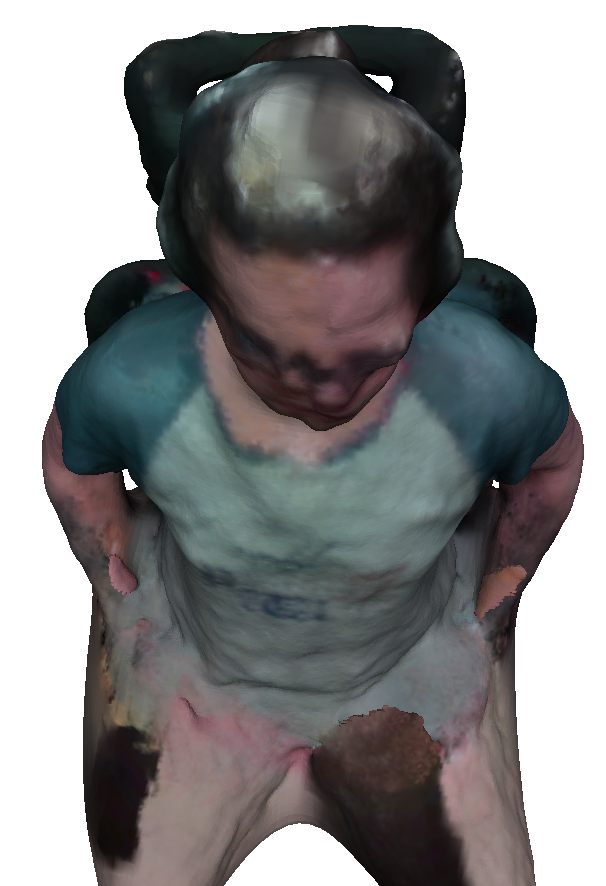
\includegraphics[height=4.5cm]{archivos/experimentacion-5-resultado-malla-5.png}
    \end{subfigure}
    \caption{Resultados de Reconstrucción 3D de un cuerpo humano usando CUDA-ICP.}
    \label{fig:resultados-reconstruccion-cuerpo-cuda}
\end{figure}

\begin{table}[h]
    \centering
      \begin{tabular}{rrrrrrrr}
            &       & \multicolumn{2}{c}{Tiempo ICP (s)} & \multicolumn{2}{c}{Tiempo CUDA-ICP (s)} & \multicolumn{2}{c}{Mejora de velocidad} \\
      \multicolumn{1}{l}{Iteración} & \multicolumn{1}{l}{Puntos} & \multicolumn{1}{l}{t/iteracion} & \multicolumn{1}{l}{Total} & \multicolumn{1}{l}{t/iteracion} & \multicolumn{1}{l}{Total} & \multicolumn{1}{l}{\%/iteración} & \multicolumn{1}{l}{Total} \\
      0     & 19256 &       &       &       &       &       &  \\
      1     & 19164 & 11,020 & 11,020 & 3,189 & 3,189 & 345,56\% & 345,56\% \\
      2     & 19021 & 18,334 & 29,354 & 5,132 & 8,321 & 357,28\% & 352,79\% \\
      3     & 19349 & 27,676 & 57,030 & 5,883 & 14,204 & 470,44\% & 401,52\% \\
      4     & 19569 & 23,892 & 80,922 & 5,165 & 19,368 & 462,62\% & 417,81\% \\
      5     & 20181 & 24,798 & 105,720 & 6,087 & 25,455 & 407,39\% & 415,32\% \\
      6     & 20137 & 34,354 & 140,074 & 5,906 & 31,361 & 581,73\% & 446,66\% \\
      7     & 19768 & 23,790 & 163,864 & 5,436 & 36,797 & 437,64\% & 445,32\% \\
      8     & 20426 & 23,262 & 187,126 & 5,517 & 42,314 & 421,64\% & 442,24\% \\
      9     & 20052 & 25,552 & 212,678 & 6,852 & 49,166 & 372,91\% & 432,58\% \\
      10    & 20626 & 20,186 & 232,864 & 5,315 & 54,480 & 379,83\% & 427,43\% \\
      11    & 20536 & 21,216 & 254,080 & 6,906 & 61,386 & 307,21\% & 413,91\% \\
      12    & 21124 & 21,516 & 275,596 & 5,096 & 66,482 & 422,25\% & 414,55\% \\
      13    & 20973 & 22,474 & 298,070 & 6,108 & 72,590 & 367,94\% & 410,62\% \\
      14    & 20902 & 42,784 & 340,854 & 7,218 & 79,808 & 592,74\% & 427,10\% \\
      15    & 21729 & 34,168 & 375,022 & 6,390 & 86,198 & 534,71\% & 435,07\% \\
      16    & 22452 & 39,848 & 414,870 & 6,783 & 92,981 & 587,47\% & 446,19\% \\
      17    & 24171 & 36,642 & 451,512 & 6,290 & 99,270 & 582,59\% & 454,83\% \\
      18    & 23220 & 28,786 & 480,298 & 8,511 & 107,781 & 338,22\% & 445,62\% \\
      19    & 22454 & 32,410 & 512,708 & 7,685 & 115,466 & 421,76\% & 444,04\% \\
      20    & 21515 & 34,930 & 547,638 & 6,904 & 122,370 & 505,90\% & 447,53\% \\
      21    & 21384 & 25,974 & 573,612 & 6,624 & 128,994 & 392,12\% & 444,68\% \\
      22    & 21760 & 32,360 & 605,972 & 8,330 & 137,324 & 388,50\% & 441,27\% \\
      23    & 21333 & 41,708 & 647,680 & 8,154 & 145,478 & 511,50\% & 445,21\% \\
      24    & 20827 & 31,954 & 679,634 & 8,511 & 153,989 & 375,44\% & 441,35\% \\
      25    & 20341 & 39,160 & 718,794 & 8,265 & 162,254 & 473,81\% & 443,01\% \\
      26    & 20055 & 33,992 & 752,786 & 8,037 & 170,291 & 422,94\% & 442,06\% \\
      27    & 19938 & 43,098 & 795,884 & 9,501 & 179,792 & 453,62\% & 442,67\% \\
      28    & 19902 & 53,970 & 849,854 & 7,707 & 187,499 & 700,27\% & 453,26\% \\
      29    & 20376 & 39,318 & 889,172 & 7,862 & 195,360 & 500,13\% & 455,15\% \\
      30    & 20385 & 50,338 & 939,510 & 9,312 & 204,672 & 540,57\% & 459,03\% \\
      31    & 19757 & 55,054 & 994,564 & 10,016 & 214,688 & 549,69\% & 463,26\% \\
    \end{tabular}%
    \caption{Resultados de Reconstrucción 3D de un cuerpo humano.}
    \label{tab:resultado-cuerpo}%
\end{table}%
  